\documentclass{beamer}
\usetheme{AnnArbor}
\usecolortheme{spruce}
\usepackage{circuitikz}
\usepackage{graphicx}
\usepackage{verbatim}

\title{ROM and Assembly}
\subtitle{Yeah so we actually made our own programming language}
\author[CMSC389E]{Akilesh Praveen | CMSC398E}
\institute{UMD}
\date{\today}

\begin{document}

    % title page
    \begin{frame}
        \titlepage
    \end{frame}
    
    % table of contents
    \begin{frame}
        \frametitle{Agenda}
        \tableofcontents
    \end{frame}
    
    \section{Announcements}
    
        \begin{frame}
                \vfill
                \centering
                \begin{beamercolorbox}[sep=8pt,center,shadow=true,rounded=true]{title}
                    \usebeamerfont{title}Announcements\par%
                \end{beamercolorbox}
                \vfill
             \end{frame}
    
        \subsection{Projects 5, 6, and 7}
        
            
            
            \begin{frame}
                \frametitle{Projects 5, 6, 7}
                \begin{itemize}
                    \item Projects 5, 6, and 7 are now released on Piazza
                    \item Relevant instructional material is/will be linked
                    \item They can be done in \textbf{any order}, but I would suggest doing them in order (5, then 6, then 7)
                    \item The next 3 lectures (including this one) are designed to help you understand the projects in that order, so stay tuned for that
                    
                \end{itemize}
            \end{frame}
            
            
    \section{ROM}
    
    	\begin{frame}
                \vfill
                \centering
                \begin{beamercolorbox}[sep=8pt,center,shadow=true,rounded=true]{title}
                    \usebeamerfont{title}Intro + Background\par%
                \end{beamercolorbox}
                \vfill
             \end{frame}
    
    		\begin{frame}
    			\frametitle{Intro}
    			\begin{itemize}
    				\item We've built the ALU; the brains of the operation
    				\item Now we need a few more things to take this from just a calculator circuit to an actual computer
    				\begin{itemize}
    					\item Ways to \textbf{store} programs
    					\item Ways to \textbf{interpret} those programs
    					\item Ways to \textbf{execute} those programs
    					\item Ways to \textbf{store data} for those programs while they're executing
    				\end{itemize}
    				\item We're going to use the digital logic circuit theory to build circuits to address all of these! (Projects 5, 6, and 7)
    			\end{itemize}
    		\end{frame}
    		
    		\begin{frame}
    			\frametitle{Intro}
    			
    				\begin{itemize}
    					\item Ways to \textbf{store} programs - \textbf{ROM} \textit{(Project 5)}
    					\item Ways to \textbf{interpret} those programs - \textbf{389E Assembly} \textit{(Project 5)}
    					\item Ways to \textbf{execute} those programs - \textbf{Program Counter} \textit{(Project 6)}
    					\item Ways to \textbf{store data} for those programs while they're executing - \textbf{RAM} \textit{(Project 7)}
    					\item Today, we'll be talking about the first two points- \textbf{storing and interpreting}.
    				\end{itemize}
    				
    			
    		\end{frame}
    		
    	\subsection{The Problem We Want to Solve}
    	
    	
    		\begin{frame}
                \vfill
                \centering
                \begin{beamercolorbox}[sep=8pt,center,shadow=true,rounded=true]{title}
                    \usebeamerfont{title}The Problem We Want to Solve\par%
                \end{beamercolorbox}
                \vfill
             \end{frame}
    	
    		\begin{frame}
    			\frametitle{The Problem We Want to Solve}
    			\begin{itemize}
    				\item Before we architect a solution, let's understand the problem we need to solve.
    				\item We need a \textbf{way to store our programs}
    				\item We need a \textbf{way to interpret our programs}
    				\item Let's start with some standard questions to help guide us there
    				\begin{itemize}
    					\item How exactly will we represent our programs?
    					\item How much space will we need?
    				\end{itemize}
    				\item Once we figure out how we'll represent our programs, we can easily develop constraints in order to store them. Once they're stored, we can tackle how we'd help our computer to interpret them.
    			\end{itemize}
    		\end{frame}
    		
    		
    		\begin{frame}
    			\frametitle{The Problem We Want to Solve}
    			\begin{itemize}
    				\item How will we represent our programs?
    				\begin{itemize}
    					\item So far, we've designed \texttt{ADD}, \texttt{SUB}, \texttt{MULT}, and other 3-bit operations. Where else have we seen basic operations like this? \textit{(Think back to 216!)}
    					\item Let's take a page out of the first programmers' books and say that we're going to write some stripped down version of assembly.
    					\item For this project, we will be working with a 14-bit version of Assembly created by the Divine for use in CMSC389E
    					\item In other words, we need \textbf{14 bits} to be able to store each instruction in CMSC389E Assembly
    				\end{itemize}
    			\end{itemize}
    		\end{frame}
    		
    		\begin{frame}
    			\frametitle{The Problem We Want to Solve}
    			\begin{itemize}
    				\item How much space will we need?
    				\begin{itemize}
    					\item That's a problem. We only have a 3-bit computer, yet our 'Assembly' will definitely take more than just 3 bits to store. (14)
    					\item We're going to use a sneaky workaround to get around this issue
    					\item Most computers store their programs in writable memory, so that they can be rewritten by the CPU, but we can drop that functionality for now
    					\item We need a way to store data larger than 3 bits so that we can fully realize our Assembly dreams. However, our computer can only manipulate 3 bits at once.
    					\item \textbf{What if} we didn't need to be able to manipulate those bits? Would that change our size constraint?
    				\end{itemize}
    			\end{itemize}
    		\end{frame}
    
    	\subsection{Our Application of ROM}
    	
    		\begin{frame}
                \vfill
                \centering
                \begin{beamercolorbox}[sep=8pt,center,shadow=true,rounded=true]{title}
                    \usebeamerfont{title}So then, Why ROM?\par%
                \end{beamercolorbox}
                \vfill
             \end{frame}
    	
    		\begin{frame}
    			\frametitle{Why ROM?}
    			\begin{itemize}
    				\item ROM is looking like a pretty good candidate for this
    				\item \textbf{Question}: Why is ROM the optimal choice for this?
    				\item Remember: our computer has a 3-bit architecture
    				\item We didn't pick read-only because it was optimal, we picked it because it's the \textit{easiest to build}
    				\item There isn't much instruction you would be able to store in 3-bit sized memory!
    				
    				
    			\end{itemize}
    			
    			{
    			\centering
    			

\tikzset{every picture/.style={line width=0.75pt}} %set default line width to 0.75pt        

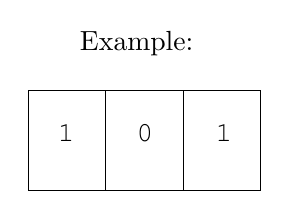
\begin{tikzpicture}[x=0.75pt,y=0.75pt,yscale=-1,xscale=1]
%uncomment if require: \path (0,300); %set diagram left start at 0, and has height of 300

%Shape: Rectangle [id:dp2530475753671312] 
\draw   (109,132.48) -- (146.33,132.48) -- (146.33,180.67) -- (109,180.67) -- cycle ;
%Shape: Rectangle [id:dp30969979889470345] 
\draw   (146.33,132.48) -- (183.67,132.48) -- (183.67,180.67) -- (146.33,180.67) -- cycle ;
%Shape: Rectangle [id:dp8255059436179499] 
\draw   (183.67,132.48) -- (221,132.48) -- (221,180.67) -- (183.67,180.67) -- cycle ;

% Text Node
\draw (122,147.67) node [anchor=north west][inner sep=0.75pt]   [align=left] {{\fontfamily{pcr}\selectfont 1}};
% Text Node
\draw (160,147.67) node [anchor=north west][inner sep=0.75pt]   [align=left] {{\fontfamily{pcr}\selectfont 0}};
% Text Node
\draw (198,147.67) node [anchor=north west][inner sep=0.75pt]   [align=left] {{\fontfamily{pcr}\selectfont 1}};
% Text Node
\draw (132.67,102.33) node [anchor=north west][inner sep=0.75pt]   [align=left] {Example:};


\end{tikzpicture}

    			}
    		\end{frame}
    		
    		\begin{frame}
    			\frametitle{The Big Idea}
    			\begin{itemize}
    				\item \textbf{BIG IDEA:} Our computer can manipulate only 3 bits at a time, and we want more than that for our programs. So, let's make it so that our computer won't have to ever manipulate the bits in our programs!
    				\begin{itemize}
    					\item \textbf{PRO:} We can store a lot more data!
    					\item \textbf{CON:} We'll have to manually edit our 'computer' to change the programs
    				\end{itemize}
    				\item This is no big problem for us though, as all we have to do is mess with a little redstone here and there if we want to 'edit' our programs.
    			\end{itemize}
    		\end{frame}
    		
    		\begin{frame}
    			\frametitle{Design: Final Thoughts}
    			\begin{itemize}
    				\item In order to represent an instruction, we want to keep it as simple as possible.
    				\item Remember, in order to \textbf{store} our Assembly-based instructions, we need 14 bits for each instruction.
    				\item 

\tikzset{every picture/.style={line width=0.75pt}} %set default line width to 0.75pt        

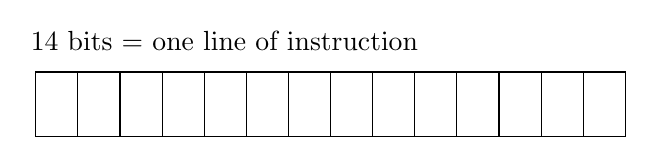
\begin{tikzpicture}[x=0.75pt,y=0.75pt,yscale=-1,xscale=1]
%uncomment if require: \path (0,300); %set diagram left start at 0, and has height of 300

%Shape: Rectangle [id:dp2530475753671312] 
\draw   (110.33,126.07) -- (130.62,126.07) -- (130.62,157.33) -- (110.33,157.33) -- cycle ;
%Shape: Rectangle [id:dp30969979889470345] 
\draw   (130.62,126.07) -- (150.9,126.07) -- (150.9,157.33) -- (130.62,157.33) -- cycle ;
%Shape: Rectangle [id:dp8255059436179499] 
\draw   (150.9,126.07) -- (171.19,126.07) -- (171.19,157.33) -- (150.9,157.33) -- cycle ;
%Shape: Rectangle [id:dp6893560723694514] 
\draw   (171.19,126.07) -- (191.48,126.07) -- (191.48,157.33) -- (171.19,157.33) -- cycle ;
%Shape: Rectangle [id:dp9841580155383872] 
\draw   (191.48,126.07) -- (211.76,126.07) -- (211.76,157.33) -- (191.48,157.33) -- cycle ;
%Shape: Rectangle [id:dp15994254936309937] 
\draw   (211.76,126.07) -- (232.05,126.07) -- (232.05,157.33) -- (211.76,157.33) -- cycle ;
%Shape: Rectangle [id:dp975217635091103] 
\draw   (232.05,126.07) -- (252.33,126.07) -- (252.33,157.33) -- (232.05,157.33) -- cycle ;
%Shape: Rectangle [id:dp060618493349726243] 
\draw   (252.33,126.07) -- (272.62,126.07) -- (272.62,157.33) -- (252.33,157.33) -- cycle ;
%Shape: Rectangle [id:dp40904506670543406] 
\draw   (272.62,126.07) -- (292.9,126.07) -- (292.9,157.33) -- (272.62,157.33) -- cycle ;
%Shape: Rectangle [id:dp8257719440129402] 
\draw   (292.9,126.07) -- (313.19,126.07) -- (313.19,157.33) -- (292.9,157.33) -- cycle ;
%Shape: Rectangle [id:dp31817883836239835] 
\draw   (313.19,126.07) -- (333.48,126.07) -- (333.48,157.33) -- (313.19,157.33) -- cycle ;
%Shape: Rectangle [id:dp3065486683425426] 
\draw   (333.48,126.07) -- (353.76,126.07) -- (353.76,157.33) -- (333.48,157.33) -- cycle ;
%Shape: Rectangle [id:dp509623912506549] 
\draw   (353.76,126.07) -- (374.05,126.07) -- (374.05,157.33) -- (353.76,157.33) -- cycle ;
%Shape: Rectangle [id:dp7886973154152628] 
\draw   (374.05,126.07) -- (394.33,126.07) -- (394.33,157.33) -- (374.05,157.33) -- cycle ;

% Text Node
\draw (106.67,105) node [anchor=north west][inner sep=0.75pt]   [align=left] {14 bits = one line of instruction};


\end{tikzpicture}

    				\item \textbf{Conclusion:} We need individual lines of read-only memory, with 14 bits in each line. This will allow us to properly \textbf{store} the programs for our computer.
    			
    			\end{itemize}
    			
    		\end{frame}
    		
    		\begin{frame}
    			\frametitle{Is space the reason why people use ROM?}
    			\begin{itemize}
    				\item Absolutely not.
    				\item Most functional computers don't have this (absurdly small) space requirement, and are perfectly able to store programs in ROM and RAM alike, as their systems are capable of manipulating more than 3 bits at a time.
    				\item However, this doesn't mean ROM is totally useless.
    				\item Some programs are better off staying in ROM rather than RAM
    				\item \textbf{Example:} The reason your computer still turns on after you wipe the disks is because the BIOS is (in most cases) a program that's been stored in ROM on your hardware.
    			
    			\end{itemize}
    			
    		\end{frame}
    		
    		
    		
    		
    	\subsection{Structure of our ROM}
    	
    		\begin{frame}
                \vfill
                \centering
                \begin{beamercolorbox}[sep=8pt,center,shadow=true,rounded=true]{title}
                    \usebeamerfont{title}The Structure of Our ROM\par%
                \end{beamercolorbox}
                \vfill
             \end{frame}
             
             \begin{frame}
                \vfill
                \centering
                \begin{beamercolorbox}[sep=8pt,center,shadow=true,rounded=true]{title}
                    \usebeamerfont{title}Storage In Minecraft\par%
                \end{beamercolorbox}
                \vfill
             \end{frame}
             
             \begin{frame}
             	\frametitle{ROM in Minecraft}
             	\begin{itemize}
             		\item Now that our memory only has to be read-only, we're set. Remember that simple read-only memory circuit we looked at? This will be even easier.
             		\item By eliminating the need to \textbf{set} and \textbf{reset} our memory, we've reduced it down to a highly simple concept.
             		\item In other words, a \texttt{1} can be as simple as a redstone torch being in a spot, and a \texttt{0} can be as simple as a redstone torch not being in that spot.
             		
             	\end{itemize}
             	
             	{
             	\centering
             	

\tikzset{every picture/.style={line width=0.75pt}} %set default line width to 0.75pt        

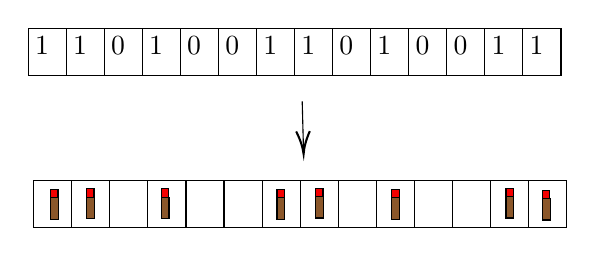
\begin{tikzpicture}[x=0.75pt,y=0.75pt,yscale=-1,xscale=1]
%uncomment if require: \path (0,300); %set diagram left start at 0, and has height of 300

%Shape: Rectangle [id:dp2530475753671312] 
\draw   (192.33,31.41) -- (210.67,31.41) -- (210.67,54) -- (192.33,54) -- cycle ;
%Shape: Rectangle [id:dp30969979889470345] 
\draw   (210.67,31.41) -- (229,31.41) -- (229,54) -- (210.67,54) -- cycle ;
%Shape: Rectangle [id:dp8255059436179499] 
\draw   (229,31.41) -- (247.33,31.41) -- (247.33,54) -- (229,54) -- cycle ;
%Shape: Rectangle [id:dp6893560723694514] 
\draw   (247.33,31.41) -- (265.67,31.41) -- (265.67,54) -- (247.33,54) -- cycle ;
%Shape: Rectangle [id:dp9841580155383872] 
\draw   (265.67,31.41) -- (284,31.41) -- (284,54) -- (265.67,54) -- cycle ;
%Shape: Rectangle [id:dp15994254936309937] 
\draw   (284,31.41) -- (302.33,31.41) -- (302.33,54) -- (284,54) -- cycle ;
%Shape: Rectangle [id:dp975217635091103] 
\draw   (302.33,31.41) -- (320.67,31.41) -- (320.67,54) -- (302.33,54) -- cycle ;
%Shape: Rectangle [id:dp060618493349726243] 
\draw   (320.67,31.41) -- (339,31.41) -- (339,54) -- (320.67,54) -- cycle ;
%Shape: Rectangle [id:dp40904506670543406] 
\draw   (339,31.41) -- (357.33,31.41) -- (357.33,54) -- (339,54) -- cycle ;
%Shape: Rectangle [id:dp8257719440129402] 
\draw   (357.33,31.41) -- (375.67,31.41) -- (375.67,54) -- (357.33,54) -- cycle ;
%Shape: Rectangle [id:dp31817883836239835] 
\draw   (375.67,31.41) -- (394,31.41) -- (394,54) -- (375.67,54) -- cycle ;
%Shape: Rectangle [id:dp3065486683425426] 
\draw   (394,31.41) -- (412.33,31.41) -- (412.33,54) -- (394,54) -- cycle ;
%Shape: Rectangle [id:dp509623912506549] 
\draw   (412.33,31.41) -- (430.67,31.41) -- (430.67,54) -- (412.33,54) -- cycle ;
%Shape: Rectangle [id:dp7886973154152628] 
\draw   (430.67,31.41) -- (449,31.41) -- (449,54) -- (430.67,54) -- cycle ;
%Straight Lines [id:da3297057722044202] 
\draw    (324.33,66.67) -- (324.95,90) ;
\draw [shift={(325,92)}, rotate = 268.49] [color={rgb, 255:red, 0; green, 0; blue, 0 }  ][line width=0.75]    (10.93,-3.29) .. controls (6.95,-1.4) and (3.31,-0.3) .. (0,0) .. controls (3.31,0.3) and (6.95,1.4) .. (10.93,3.29)   ;
%Shape: Rectangle [id:dp7306471770838919] 
\draw   (195,104.74) -- (213.33,104.74) -- (213.33,127.33) -- (195,127.33) -- cycle ;
%Shape: Rectangle [id:dp5607628345341253] 
\draw   (213.33,104.74) -- (231.67,104.74) -- (231.67,127.33) -- (213.33,127.33) -- cycle ;
%Shape: Rectangle [id:dp0792661956068278] 
\draw   (231.67,104.74) -- (250,104.74) -- (250,127.33) -- (231.67,127.33) -- cycle ;
%Shape: Rectangle [id:dp8623895262875295] 
\draw   (250,104.74) -- (268.33,104.74) -- (268.33,127.33) -- (250,127.33) -- cycle ;
%Shape: Rectangle [id:dp009175660727291923] 
\draw   (268.33,104.74) -- (286.67,104.74) -- (286.67,127.33) -- (268.33,127.33) -- cycle ;
%Shape: Rectangle [id:dp4729260459269564] 
\draw   (286.67,104.74) -- (305,104.74) -- (305,127.33) -- (286.67,127.33) -- cycle ;
%Shape: Rectangle [id:dp4530702176374507] 
\draw   (305,104.74) -- (323.33,104.74) -- (323.33,127.33) -- (305,127.33) -- cycle ;
%Shape: Rectangle [id:dp18274736433593486] 
\draw   (323.33,104.74) -- (341.67,104.74) -- (341.67,127.33) -- (323.33,127.33) -- cycle ;
%Shape: Rectangle [id:dp6454813939338947] 
\draw   (341.67,104.74) -- (360,104.74) -- (360,127.33) -- (341.67,127.33) -- cycle ;
%Shape: Rectangle [id:dp44415589930378796] 
\draw   (360,104.74) -- (378.33,104.74) -- (378.33,127.33) -- (360,127.33) -- cycle ;
%Shape: Rectangle [id:dp44316809627896814] 
\draw   (378.33,104.74) -- (396.67,104.74) -- (396.67,127.33) -- (378.33,127.33) -- cycle ;
%Shape: Rectangle [id:dp3768823609089883] 
\draw   (396.67,104.74) -- (415,104.74) -- (415,127.33) -- (396.67,127.33) -- cycle ;
%Shape: Rectangle [id:dp2370210201858336] 
\draw   (415,104.74) -- (433.33,104.74) -- (433.33,127.33) -- (415,127.33) -- cycle ;
%Shape: Rectangle [id:dp4899807962812457] 
\draw   (433.33,104.74) -- (451.67,104.74) -- (451.67,127.33) -- (433.33,127.33) -- cycle ;
%Shape: Rectangle [id:dp4368680678750193] 
\draw  [fill={rgb, 255:red, 139; green, 87; blue, 42 }  ,fill opacity=1 ] (203.17,113.08) -- (206.83,113.08) -- (206.83,123.5) -- (203.17,123.5) -- cycle ;
%Shape: Rectangle [id:dp09500539877263525] 
\draw  [fill={rgb, 255:red, 244; green, 0; blue, 0 }  ,fill opacity=1 ] (203.17,109.17) -- (206.67,109.17) -- (206.67,113.08) -- (203.17,113.08) -- cycle ;
%Shape: Rectangle [id:dp1483728050123183] 
\draw  [fill={rgb, 255:red, 139; green, 87; blue, 42 }  ,fill opacity=1 ] (220.5,112.75) -- (224.17,112.75) -- (224.17,123.17) -- (220.5,123.17) -- cycle ;
%Shape: Rectangle [id:dp593349582542728] 
\draw  [fill={rgb, 255:red, 244; green, 0; blue, 0 }  ,fill opacity=1 ] (220.5,108.83) -- (224,108.83) -- (224,112.75) -- (220.5,112.75) -- cycle ;
%Shape: Rectangle [id:dp4070158701487039] 
\draw  [fill={rgb, 255:red, 139; green, 87; blue, 42 }  ,fill opacity=1 ] (256.5,112.75) -- (260.17,112.75) -- (260.17,123.17) -- (256.5,123.17) -- cycle ;
%Shape: Rectangle [id:dp4458058453343535] 
\draw  [fill={rgb, 255:red, 244; green, 0; blue, 0 }  ,fill opacity=1 ] (256.5,108.83) -- (260,108.83) -- (260,112.75) -- (256.5,112.75) -- cycle ;
%Shape: Rectangle [id:dp9277371430125845] 
\draw  [fill={rgb, 255:red, 139; green, 87; blue, 42 }  ,fill opacity=1 ] (440.17,113.42) -- (443.83,113.42) -- (443.83,123.83) -- (440.17,123.83) -- cycle ;
%Shape: Rectangle [id:dp3082228602345055] 
\draw  [fill={rgb, 255:red, 244; green, 0; blue, 0 }  ,fill opacity=1 ] (440.17,109.5) -- (443.67,109.5) -- (443.67,113.42) -- (440.17,113.42) -- cycle ;
%Shape: Rectangle [id:dp17154116631501037] 
\draw  [fill={rgb, 255:red, 139; green, 87; blue, 42 }  ,fill opacity=1 ] (312.17,113.08) -- (315.83,113.08) -- (315.83,123.5) -- (312.17,123.5) -- cycle ;
%Shape: Rectangle [id:dp6278512827702475] 
\draw  [fill={rgb, 255:red, 244; green, 0; blue, 0 }  ,fill opacity=1 ] (312.17,109.17) -- (315.67,109.17) -- (315.67,113.08) -- (312.17,113.08) -- cycle ;
%Shape: Rectangle [id:dp31389089597210484] 
\draw  [fill={rgb, 255:red, 139; green, 87; blue, 42 }  ,fill opacity=1 ] (330.83,112.42) -- (334.5,112.42) -- (334.5,122.83) -- (330.83,122.83) -- cycle ;
%Shape: Rectangle [id:dp3848680259197699] 
\draw  [fill={rgb, 255:red, 244; green, 0; blue, 0 }  ,fill opacity=1 ] (330.83,108.5) -- (334.33,108.5) -- (334.33,112.42) -- (330.83,112.42) -- cycle ;
%Shape: Rectangle [id:dp6018543086688013] 
\draw  [fill={rgb, 255:red, 139; green, 87; blue, 42 }  ,fill opacity=1 ] (367.5,113.08) -- (371.17,113.08) -- (371.17,123.5) -- (367.5,123.5) -- cycle ;
%Shape: Rectangle [id:dp599252549604423] 
\draw  [fill={rgb, 255:red, 244; green, 0; blue, 0 }  ,fill opacity=1 ] (367.5,109.17) -- (371,109.17) -- (371,113.08) -- (367.5,113.08) -- cycle ;
%Shape: Rectangle [id:dp9476241971366911] 
\draw  [fill={rgb, 255:red, 139; green, 87; blue, 42 }  ,fill opacity=1 ] (422.5,112.42) -- (426.17,112.42) -- (426.17,122.83) -- (422.5,122.83) -- cycle ;
%Shape: Rectangle [id:dp6884535278941168] 
\draw  [fill={rgb, 255:red, 244; green, 0; blue, 0 }  ,fill opacity=1 ] (422.5,108.5) -- (426,108.5) -- (426,112.42) -- (422.5,112.42) -- cycle ;

% Text Node
\draw (194.33,34.41) node [anchor=north west][inner sep=0.75pt]   [align=left] {1};
% Text Node
\draw (212.67,34.41) node [anchor=north west][inner sep=0.75pt]   [align=left] {1};
% Text Node
\draw (304.33,34.41) node [anchor=north west][inner sep=0.75pt]   [align=left] {1};
% Text Node
\draw (249.33,34.41) node [anchor=north west][inner sep=0.75pt]   [align=left] {1};
% Text Node
\draw (267.67,34.41) node [anchor=north west][inner sep=0.75pt]   [align=left] {0};
% Text Node
\draw (286,34.41) node [anchor=north west][inner sep=0.75pt]   [align=left] {0};
% Text Node
\draw (341,34.41) node [anchor=north west][inner sep=0.75pt]   [align=left] {0};
% Text Node
\draw (377.67,34.41) node [anchor=north west][inner sep=0.75pt]   [align=left] {0};
% Text Node
\draw (396,34.41) node [anchor=north west][inner sep=0.75pt]   [align=left] {0};
% Text Node
\draw (231,34.41) node [anchor=north west][inner sep=0.75pt]   [align=left] {0};
% Text Node
\draw (322.67,34.41) node [anchor=north west][inner sep=0.75pt]   [align=left] {1};
% Text Node
\draw (359.33,34.41) node [anchor=north west][inner sep=0.75pt]   [align=left] {1};
% Text Node
\draw (414.33,34.41) node [anchor=north west][inner sep=0.75pt]   [align=left] {1};
% Text Node
\draw (432.67,34.41) node [anchor=north west][inner sep=0.75pt]   [align=left] {1};


\end{tikzpicture}

             	}
             \end{frame}
             
             \begin{frame}
             	\frametitle{ROM in Minecraft}
             	\begin{itemize}
             		\item We can figure out what each line is saying by running some redstone wire under these blocks, in order to pick up the output of the torches.
             	\end{itemize}
             	
             	{
             	\centering
             	

\tikzset{every picture/.style={line width=0.75pt}} %set default line width to 0.75pt        

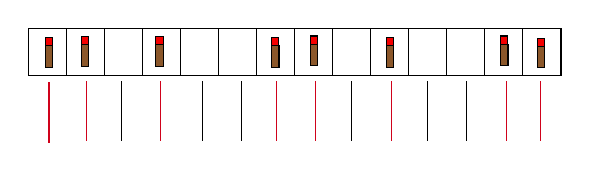
\begin{tikzpicture}[x=0.75pt,y=0.75pt,yscale=-1,xscale=1]
%uncomment if require: \path (0,300); %set diagram left start at 0, and has height of 300

%Shape: Rectangle [id:dp7306471770838919] 
\draw   (195,104.74) -- (213.33,104.74) -- (213.33,127.33) -- (195,127.33) -- cycle ;
%Shape: Rectangle [id:dp5607628345341253] 
\draw   (213.33,104.74) -- (231.67,104.74) -- (231.67,127.33) -- (213.33,127.33) -- cycle ;
%Shape: Rectangle [id:dp0792661956068278] 
\draw   (231.67,104.74) -- (250,104.74) -- (250,127.33) -- (231.67,127.33) -- cycle ;
%Shape: Rectangle [id:dp8623895262875295] 
\draw   (250,104.74) -- (268.33,104.74) -- (268.33,127.33) -- (250,127.33) -- cycle ;
%Shape: Rectangle [id:dp009175660727291923] 
\draw   (268.33,104.74) -- (286.67,104.74) -- (286.67,127.33) -- (268.33,127.33) -- cycle ;
%Shape: Rectangle [id:dp4729260459269564] 
\draw   (286.67,104.74) -- (305,104.74) -- (305,127.33) -- (286.67,127.33) -- cycle ;
%Shape: Rectangle [id:dp4530702176374507] 
\draw   (305,104.74) -- (323.33,104.74) -- (323.33,127.33) -- (305,127.33) -- cycle ;
%Shape: Rectangle [id:dp18274736433593486] 
\draw   (323.33,104.74) -- (341.67,104.74) -- (341.67,127.33) -- (323.33,127.33) -- cycle ;
%Shape: Rectangle [id:dp6454813939338947] 
\draw   (341.67,104.74) -- (360,104.74) -- (360,127.33) -- (341.67,127.33) -- cycle ;
%Shape: Rectangle [id:dp44415589930378796] 
\draw   (360,104.74) -- (378.33,104.74) -- (378.33,127.33) -- (360,127.33) -- cycle ;
%Shape: Rectangle [id:dp44316809627896814] 
\draw   (378.33,104.74) -- (396.67,104.74) -- (396.67,127.33) -- (378.33,127.33) -- cycle ;
%Shape: Rectangle [id:dp3768823609089883] 
\draw   (396.67,104.74) -- (415,104.74) -- (415,127.33) -- (396.67,127.33) -- cycle ;
%Shape: Rectangle [id:dp2370210201858336] 
\draw   (415,104.74) -- (433.33,104.74) -- (433.33,127.33) -- (415,127.33) -- cycle ;
%Shape: Rectangle [id:dp4899807962812457] 
\draw   (433.33,104.74) -- (451.67,104.74) -- (451.67,127.33) -- (433.33,127.33) -- cycle ;
%Shape: Rectangle [id:dp4368680678750193] 
\draw  [fill={rgb, 255:red, 139; green, 87; blue, 42 }  ,fill opacity=1 ] (203.17,113.08) -- (206.83,113.08) -- (206.83,123.5) -- (203.17,123.5) -- cycle ;
%Shape: Rectangle [id:dp09500539877263525] 
\draw  [fill={rgb, 255:red, 244; green, 0; blue, 0 }  ,fill opacity=1 ] (203.17,109.17) -- (206.67,109.17) -- (206.67,113.08) -- (203.17,113.08) -- cycle ;
%Shape: Rectangle [id:dp1483728050123183] 
\draw  [fill={rgb, 255:red, 139; green, 87; blue, 42 }  ,fill opacity=1 ] (220.5,112.75) -- (224.17,112.75) -- (224.17,123.17) -- (220.5,123.17) -- cycle ;
%Shape: Rectangle [id:dp593349582542728] 
\draw  [fill={rgb, 255:red, 244; green, 0; blue, 0 }  ,fill opacity=1 ] (220.5,108.83) -- (224,108.83) -- (224,112.75) -- (220.5,112.75) -- cycle ;
%Shape: Rectangle [id:dp4070158701487039] 
\draw  [fill={rgb, 255:red, 139; green, 87; blue, 42 }  ,fill opacity=1 ] (256.5,112.75) -- (260.17,112.75) -- (260.17,123.17) -- (256.5,123.17) -- cycle ;
%Shape: Rectangle [id:dp4458058453343535] 
\draw  [fill={rgb, 255:red, 244; green, 0; blue, 0 }  ,fill opacity=1 ] (256.5,108.83) -- (260,108.83) -- (260,112.75) -- (256.5,112.75) -- cycle ;
%Shape: Rectangle [id:dp9277371430125845] 
\draw  [fill={rgb, 255:red, 139; green, 87; blue, 42 }  ,fill opacity=1 ] (440.17,113.42) -- (443.83,113.42) -- (443.83,123.83) -- (440.17,123.83) -- cycle ;
%Shape: Rectangle [id:dp3082228602345055] 
\draw  [fill={rgb, 255:red, 244; green, 0; blue, 0 }  ,fill opacity=1 ] (440.17,109.5) -- (443.67,109.5) -- (443.67,113.42) -- (440.17,113.42) -- cycle ;
%Shape: Rectangle [id:dp17154116631501037] 
\draw  [fill={rgb, 255:red, 139; green, 87; blue, 42 }  ,fill opacity=1 ] (312.17,113.08) -- (315.83,113.08) -- (315.83,123.5) -- (312.17,123.5) -- cycle ;
%Shape: Rectangle [id:dp6278512827702475] 
\draw  [fill={rgb, 255:red, 244; green, 0; blue, 0 }  ,fill opacity=1 ] (312.17,109.17) -- (315.67,109.17) -- (315.67,113.08) -- (312.17,113.08) -- cycle ;
%Shape: Rectangle [id:dp31389089597210484] 
\draw  [fill={rgb, 255:red, 139; green, 87; blue, 42 }  ,fill opacity=1 ] (330.83,112.42) -- (334.5,112.42) -- (334.5,122.83) -- (330.83,122.83) -- cycle ;
%Shape: Rectangle [id:dp3848680259197699] 
\draw  [fill={rgb, 255:red, 244; green, 0; blue, 0 }  ,fill opacity=1 ] (330.83,108.5) -- (334.33,108.5) -- (334.33,112.42) -- (330.83,112.42) -- cycle ;
%Shape: Rectangle [id:dp6018543086688013] 
\draw  [fill={rgb, 255:red, 139; green, 87; blue, 42 }  ,fill opacity=1 ] (367.5,113.08) -- (371.17,113.08) -- (371.17,123.5) -- (367.5,123.5) -- cycle ;
%Shape: Rectangle [id:dp599252549604423] 
\draw  [fill={rgb, 255:red, 244; green, 0; blue, 0 }  ,fill opacity=1 ] (367.5,109.17) -- (371,109.17) -- (371,113.08) -- (367.5,113.08) -- cycle ;
%Shape: Rectangle [id:dp9476241971366911] 
\draw  [fill={rgb, 255:red, 139; green, 87; blue, 42 }  ,fill opacity=1 ] (422.5,112.42) -- (426.17,112.42) -- (426.17,122.83) -- (422.5,122.83) -- cycle ;
%Shape: Rectangle [id:dp6884535278941168] 
\draw  [fill={rgb, 255:red, 244; green, 0; blue, 0 }  ,fill opacity=1 ] (422.5,108.5) -- (426,108.5) -- (426,112.42) -- (422.5,112.42) -- cycle ;
%Straight Lines [id:da8130436103927301] 
\draw [color={rgb, 255:red, 208; green, 2; blue, 27 }  ,draw opacity=1 ]   (205,130.83) -- (205,159.83) ;
%Straight Lines [id:da08462131345193069] 
\draw [color={rgb, 255:red, 208; green, 2; blue, 27 }  ,draw opacity=1 ]   (223,130.17) -- (223,159.17) ;
%Straight Lines [id:da8359957829774382] 
\draw [color={rgb, 255:red, 208; green, 2; blue, 27 }  ,draw opacity=1 ]   (258.67,130.17) -- (258.67,159.17) ;
%Straight Lines [id:da3866920597345579] 
\draw [color={rgb, 255:red, 208; green, 2; blue, 27 }  ,draw opacity=1 ]   (314.67,130.17) -- (314.67,159.17) ;
%Straight Lines [id:da5942403939779883] 
\draw [color={rgb, 255:red, 208; green, 2; blue, 27 }  ,draw opacity=1 ]   (333.33,130.17) -- (333.33,159.17) ;
%Straight Lines [id:da22634310425539206] 
\draw [color={rgb, 255:red, 208; green, 2; blue, 27 }  ,draw opacity=1 ]   (370,130.17) -- (370,159.17) ;
%Straight Lines [id:da23791169110885224] 
\draw [color={rgb, 255:red, 208; green, 2; blue, 27 }  ,draw opacity=1 ]   (425.33,130.17) -- (425.33,159.17) ;
%Straight Lines [id:da9365841080673278] 
\draw [color={rgb, 255:red, 208; green, 2; blue, 27 }  ,draw opacity=1 ]   (441.67,130.17) -- (441.67,159.17) ;
%Straight Lines [id:da3945985170381383] 
\draw [color={rgb, 255:red, 0; green, 0; blue, 0 }  ,draw opacity=1 ]   (240,130.17) -- (240,159.17) ;
%Straight Lines [id:da3721123428333971] 
\draw [color={rgb, 255:red, 0; green, 0; blue, 0 }  ,draw opacity=1 ]   (279,130.17) -- (279,159.17) ;
%Straight Lines [id:da013616551740032623] 
\draw [color={rgb, 255:red, 0; green, 0; blue, 0 }  ,draw opacity=1 ]   (297.67,130.17) -- (297.67,159.17) ;
%Straight Lines [id:da9364095553547536] 
\draw [color={rgb, 255:red, 0; green, 0; blue, 0 }  ,draw opacity=1 ]   (350.67,130.17) -- (350.67,159.17) ;
%Straight Lines [id:da7903503951079389] 
\draw [color={rgb, 255:red, 0; green, 0; blue, 0 }  ,draw opacity=1 ]   (387.33,130.17) -- (387.33,159.17) ;
%Straight Lines [id:da6948026493349652] 
\draw [color={rgb, 255:red, 0; green, 0; blue, 0 }  ,draw opacity=1 ]   (406,130.17) -- (406,159.17) ;




\end{tikzpicture}

             	}
             	
             \end{frame}
             
             \begin{frame}
             	\frametitle{ROM in Minecraft}
             	\begin{itemize}
             		\item Now we have an idea of how to write a 'line' of our CMSC389E assembly
             		\item Forget about the actual rules of the assembly for now, let's just be pleased with the fact that we've figured out how to represent a line of 0's and 1's within Minecraft
             		\item Now here's another question. This is just one line. How can we represent different lines?
             	\end{itemize}
             	
             	{
             	\centering
             	
             	}
             \end{frame}
             
             \begin{frame}
             	\frametitle{ROM in Minecraft}
             	\begin{itemize}
             		\item Now we have an idea of how to write a 'line' of our CMSC389E assembly
             		\item Forget about the actual rules of the assembly for now, let's just be pleased with the fact that we've figured out how to represent a line of 0's and 1's within Minecraft
             		\item Now here's another question. This is just one line. How can we represent different lines?
             		\item \textbf{Answer: It's quite simple. We make more 'lines'}
             	\end{itemize}
             	
             	{
             	\centering
             	

\tikzset{every picture/.style={line width=0.75pt}} %set default line width to 0.75pt        

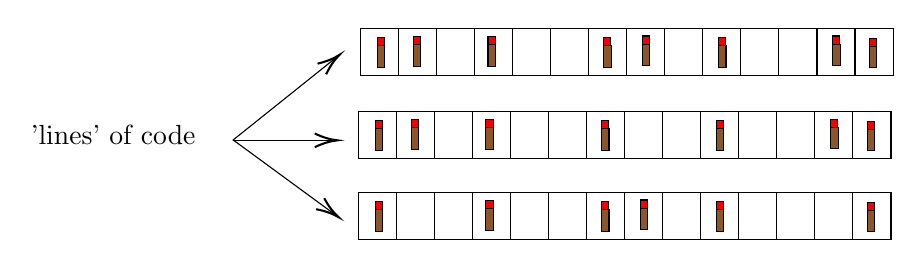
\begin{tikzpicture}[x=0.75pt,y=0.75pt,yscale=-1,xscale=1]
%uncomment if require: \path (0,300); %set diagram left start at 0, and has height of 300

%Shape: Rectangle [id:dp7306471770838919] 
\draw   (193.5,103.24) -- (211.83,103.24) -- (211.83,125.83) -- (193.5,125.83) -- cycle ;
%Shape: Rectangle [id:dp5607628345341253] 
\draw   (211.83,103.24) -- (230.17,103.24) -- (230.17,125.83) -- (211.83,125.83) -- cycle ;
%Shape: Rectangle [id:dp0792661956068278] 
\draw   (230.17,103.24) -- (248.5,103.24) -- (248.5,125.83) -- (230.17,125.83) -- cycle ;
%Shape: Rectangle [id:dp8623895262875295] 
\draw   (248.5,103.24) -- (266.83,103.24) -- (266.83,125.83) -- (248.5,125.83) -- cycle ;
%Shape: Rectangle [id:dp009175660727291923] 
\draw   (266.83,103.24) -- (285.17,103.24) -- (285.17,125.83) -- (266.83,125.83) -- cycle ;
%Shape: Rectangle [id:dp4729260459269564] 
\draw   (285.17,103.24) -- (303.5,103.24) -- (303.5,125.83) -- (285.17,125.83) -- cycle ;
%Shape: Rectangle [id:dp4530702176374507] 
\draw   (303.5,103.24) -- (321.83,103.24) -- (321.83,125.83) -- (303.5,125.83) -- cycle ;
%Shape: Rectangle [id:dp18274736433593486] 
\draw   (321.83,103.24) -- (340.17,103.24) -- (340.17,125.83) -- (321.83,125.83) -- cycle ;
%Shape: Rectangle [id:dp6454813939338947] 
\draw   (340.17,103.24) -- (358.5,103.24) -- (358.5,125.83) -- (340.17,125.83) -- cycle ;
%Shape: Rectangle [id:dp44415589930378796] 
\draw   (358.5,103.24) -- (376.83,103.24) -- (376.83,125.83) -- (358.5,125.83) -- cycle ;
%Shape: Rectangle [id:dp44316809627896814] 
\draw   (376.83,103.24) -- (395.17,103.24) -- (395.17,125.83) -- (376.83,125.83) -- cycle ;
%Shape: Rectangle [id:dp3768823609089883] 
\draw   (395.17,103.24) -- (413.5,103.24) -- (413.5,125.83) -- (395.17,125.83) -- cycle ;
%Shape: Rectangle [id:dp2370210201858336] 
\draw   (413.5,103.24) -- (431.83,103.24) -- (431.83,125.83) -- (413.5,125.83) -- cycle ;
%Shape: Rectangle [id:dp4899807962812457] 
\draw   (431.83,103.24) -- (450.17,103.24) -- (450.17,125.83) -- (431.83,125.83) -- cycle ;
%Shape: Rectangle [id:dp4368680678750193] 
\draw  [fill={rgb, 255:red, 139; green, 87; blue, 42 }  ,fill opacity=1 ] (201.67,111.58) -- (205.33,111.58) -- (205.33,122) -- (201.67,122) -- cycle ;
%Shape: Rectangle [id:dp09500539877263525] 
\draw  [fill={rgb, 255:red, 244; green, 0; blue, 0 }  ,fill opacity=1 ] (201.67,107.67) -- (205.17,107.67) -- (205.17,111.58) -- (201.67,111.58) -- cycle ;
%Shape: Rectangle [id:dp1483728050123183] 
\draw  [fill={rgb, 255:red, 139; green, 87; blue, 42 }  ,fill opacity=1 ] (219,111.25) -- (222.67,111.25) -- (222.67,121.67) -- (219,121.67) -- cycle ;
%Shape: Rectangle [id:dp593349582542728] 
\draw  [fill={rgb, 255:red, 244; green, 0; blue, 0 }  ,fill opacity=1 ] (219,107.33) -- (222.5,107.33) -- (222.5,111.25) -- (219,111.25) -- cycle ;
%Shape: Rectangle [id:dp4070158701487039] 
\draw  [fill={rgb, 255:red, 139; green, 87; blue, 42 }  ,fill opacity=1 ] (255,111.25) -- (258.67,111.25) -- (258.67,121.67) -- (255,121.67) -- cycle ;
%Shape: Rectangle [id:dp4458058453343535] 
\draw  [fill={rgb, 255:red, 244; green, 0; blue, 0 }  ,fill opacity=1 ] (255,107.33) -- (258.5,107.33) -- (258.5,111.25) -- (255,111.25) -- cycle ;
%Shape: Rectangle [id:dp9277371430125845] 
\draw  [fill={rgb, 255:red, 139; green, 87; blue, 42 }  ,fill opacity=1 ] (438.67,111.92) -- (442.33,111.92) -- (442.33,122.33) -- (438.67,122.33) -- cycle ;
%Shape: Rectangle [id:dp3082228602345055] 
\draw  [fill={rgb, 255:red, 244; green, 0; blue, 0 }  ,fill opacity=1 ] (438.67,108) -- (442.17,108) -- (442.17,111.92) -- (438.67,111.92) -- cycle ;
%Shape: Rectangle [id:dp17154116631501037] 
\draw  [fill={rgb, 255:red, 139; green, 87; blue, 42 }  ,fill opacity=1 ] (310.67,111.58) -- (314.33,111.58) -- (314.33,122) -- (310.67,122) -- cycle ;
%Shape: Rectangle [id:dp6278512827702475] 
\draw  [fill={rgb, 255:red, 244; green, 0; blue, 0 }  ,fill opacity=1 ] (310.67,107.67) -- (314.17,107.67) -- (314.17,111.58) -- (310.67,111.58) -- cycle ;
%Shape: Rectangle [id:dp31389089597210484] 
\draw  [fill={rgb, 255:red, 139; green, 87; blue, 42 }  ,fill opacity=1 ] (329.33,110.92) -- (333,110.92) -- (333,121.33) -- (329.33,121.33) -- cycle ;
%Shape: Rectangle [id:dp3848680259197699] 
\draw  [fill={rgb, 255:red, 244; green, 0; blue, 0 }  ,fill opacity=1 ] (329.33,107) -- (332.83,107) -- (332.83,110.92) -- (329.33,110.92) -- cycle ;
%Shape: Rectangle [id:dp6018543086688013] 
\draw  [fill={rgb, 255:red, 139; green, 87; blue, 42 }  ,fill opacity=1 ] (366,111.58) -- (369.67,111.58) -- (369.67,122) -- (366,122) -- cycle ;
%Shape: Rectangle [id:dp599252549604423] 
\draw  [fill={rgb, 255:red, 244; green, 0; blue, 0 }  ,fill opacity=1 ] (366,107.67) -- (369.5,107.67) -- (369.5,111.58) -- (366,111.58) -- cycle ;
%Shape: Rectangle [id:dp9476241971366911] 
\draw  [fill={rgb, 255:red, 139; green, 87; blue, 42 }  ,fill opacity=1 ] (421,110.92) -- (424.67,110.92) -- (424.67,121.33) -- (421,121.33) -- cycle ;
%Shape: Rectangle [id:dp6884535278941168] 
\draw  [fill={rgb, 255:red, 244; green, 0; blue, 0 }  ,fill opacity=1 ] (421,107) -- (424.5,107) -- (424.5,110.92) -- (421,110.92) -- cycle ;
%Shape: Rectangle [id:dp21310684225387844] 
\draw   (192.5,143.24) -- (210.83,143.24) -- (210.83,165.83) -- (192.5,165.83) -- cycle ;
%Shape: Rectangle [id:dp15308541080894023] 
\draw   (210.83,143.24) -- (229.17,143.24) -- (229.17,165.83) -- (210.83,165.83) -- cycle ;
%Shape: Rectangle [id:dp7369128603266555] 
\draw   (229.17,143.24) -- (247.5,143.24) -- (247.5,165.83) -- (229.17,165.83) -- cycle ;
%Shape: Rectangle [id:dp08559110440629836] 
\draw   (247.5,143.24) -- (265.83,143.24) -- (265.83,165.83) -- (247.5,165.83) -- cycle ;
%Shape: Rectangle [id:dp14775457548619686] 
\draw   (265.83,143.24) -- (284.17,143.24) -- (284.17,165.83) -- (265.83,165.83) -- cycle ;
%Shape: Rectangle [id:dp3380965502807922] 
\draw   (284.17,143.24) -- (302.5,143.24) -- (302.5,165.83) -- (284.17,165.83) -- cycle ;
%Shape: Rectangle [id:dp04351713499783527] 
\draw   (302.5,143.24) -- (320.83,143.24) -- (320.83,165.83) -- (302.5,165.83) -- cycle ;
%Shape: Rectangle [id:dp13842235101866918] 
\draw   (320.83,143.24) -- (339.17,143.24) -- (339.17,165.83) -- (320.83,165.83) -- cycle ;
%Shape: Rectangle [id:dp899528791244269] 
\draw   (339.17,143.24) -- (357.5,143.24) -- (357.5,165.83) -- (339.17,165.83) -- cycle ;
%Shape: Rectangle [id:dp6918354352356124] 
\draw   (357.5,143.24) -- (375.83,143.24) -- (375.83,165.83) -- (357.5,165.83) -- cycle ;
%Shape: Rectangle [id:dp25235294258499197] 
\draw   (375.83,143.24) -- (394.17,143.24) -- (394.17,165.83) -- (375.83,165.83) -- cycle ;
%Shape: Rectangle [id:dp28869943259524966] 
\draw   (394.17,143.24) -- (412.5,143.24) -- (412.5,165.83) -- (394.17,165.83) -- cycle ;
%Shape: Rectangle [id:dp07934088847037046] 
\draw   (412.5,143.24) -- (430.83,143.24) -- (430.83,165.83) -- (412.5,165.83) -- cycle ;
%Shape: Rectangle [id:dp46470597708034844] 
\draw   (430.83,143.24) -- (449.17,143.24) -- (449.17,165.83) -- (430.83,165.83) -- cycle ;
%Shape: Rectangle [id:dp04901031477430984] 
\draw  [fill={rgb, 255:red, 139; green, 87; blue, 42 }  ,fill opacity=1 ] (200.67,151.58) -- (204.33,151.58) -- (204.33,162) -- (200.67,162) -- cycle ;
%Shape: Rectangle [id:dp24013735270779224] 
\draw  [fill={rgb, 255:red, 244; green, 0; blue, 0 }  ,fill opacity=1 ] (200.67,147.67) -- (204.17,147.67) -- (204.17,151.58) -- (200.67,151.58) -- cycle ;
%Shape: Rectangle [id:dp3732303325269448] 
\draw  [fill={rgb, 255:red, 139; green, 87; blue, 42 }  ,fill opacity=1 ] (218,151.25) -- (221.67,151.25) -- (221.67,161.67) -- (218,161.67) -- cycle ;
%Shape: Rectangle [id:dp2562802987887275] 
\draw  [fill={rgb, 255:red, 244; green, 0; blue, 0 }  ,fill opacity=1 ] (218,147.33) -- (221.5,147.33) -- (221.5,151.25) -- (218,151.25) -- cycle ;
%Shape: Rectangle [id:dp9262202162888669] 
\draw  [fill={rgb, 255:red, 139; green, 87; blue, 42 }  ,fill opacity=1 ] (254,151.25) -- (257.67,151.25) -- (257.67,161.67) -- (254,161.67) -- cycle ;
%Shape: Rectangle [id:dp7111698984131953] 
\draw  [fill={rgb, 255:red, 244; green, 0; blue, 0 }  ,fill opacity=1 ] (254,147.33) -- (257.5,147.33) -- (257.5,151.25) -- (254,151.25) -- cycle ;
%Shape: Rectangle [id:dp6100628938411732] 
\draw  [fill={rgb, 255:red, 139; green, 87; blue, 42 }  ,fill opacity=1 ] (437.67,151.92) -- (441.33,151.92) -- (441.33,162.33) -- (437.67,162.33) -- cycle ;
%Shape: Rectangle [id:dp3984678192626203] 
\draw  [fill={rgb, 255:red, 244; green, 0; blue, 0 }  ,fill opacity=1 ] (437.67,148) -- (441.17,148) -- (441.17,151.92) -- (437.67,151.92) -- cycle ;
%Shape: Rectangle [id:dp5088329182863778] 
\draw  [fill={rgb, 255:red, 139; green, 87; blue, 42 }  ,fill opacity=1 ] (309.67,151.58) -- (313.33,151.58) -- (313.33,162) -- (309.67,162) -- cycle ;
%Shape: Rectangle [id:dp7660558191775368] 
\draw  [fill={rgb, 255:red, 244; green, 0; blue, 0 }  ,fill opacity=1 ] (309.67,147.67) -- (313.17,147.67) -- (313.17,151.58) -- (309.67,151.58) -- cycle ;
%Shape: Rectangle [id:dp6967450219158551] 
\draw  [fill={rgb, 255:red, 139; green, 87; blue, 42 }  ,fill opacity=1 ] (365,151.58) -- (368.67,151.58) -- (368.67,162) -- (365,162) -- cycle ;
%Shape: Rectangle [id:dp2672105385631931] 
\draw  [fill={rgb, 255:red, 244; green, 0; blue, 0 }  ,fill opacity=1 ] (365,147.67) -- (368.5,147.67) -- (368.5,151.58) -- (365,151.58) -- cycle ;
%Shape: Rectangle [id:dp1772934340190394] 
\draw  [fill={rgb, 255:red, 139; green, 87; blue, 42 }  ,fill opacity=1 ] (420,150.92) -- (423.67,150.92) -- (423.67,161.33) -- (420,161.33) -- cycle ;
%Shape: Rectangle [id:dp33718367695896434] 
\draw  [fill={rgb, 255:red, 244; green, 0; blue, 0 }  ,fill opacity=1 ] (420,147) -- (423.5,147) -- (423.5,150.92) -- (420,150.92) -- cycle ;
%Shape: Rectangle [id:dp29973241992445065] 
\draw   (192.5,182.24) -- (210.83,182.24) -- (210.83,204.83) -- (192.5,204.83) -- cycle ;
%Shape: Rectangle [id:dp915797441388662] 
\draw   (210.83,182.24) -- (229.17,182.24) -- (229.17,204.83) -- (210.83,204.83) -- cycle ;
%Shape: Rectangle [id:dp6972498895193435] 
\draw   (229.17,182.24) -- (247.5,182.24) -- (247.5,204.83) -- (229.17,204.83) -- cycle ;
%Shape: Rectangle [id:dp5185032478559118] 
\draw   (247.5,182.24) -- (265.83,182.24) -- (265.83,204.83) -- (247.5,204.83) -- cycle ;
%Shape: Rectangle [id:dp8211606146424363] 
\draw   (265.83,182.24) -- (284.17,182.24) -- (284.17,204.83) -- (265.83,204.83) -- cycle ;
%Shape: Rectangle [id:dp8023896256315195] 
\draw   (284.17,182.24) -- (302.5,182.24) -- (302.5,204.83) -- (284.17,204.83) -- cycle ;
%Shape: Rectangle [id:dp49891219038392] 
\draw   (302.5,182.24) -- (320.83,182.24) -- (320.83,204.83) -- (302.5,204.83) -- cycle ;
%Shape: Rectangle [id:dp6600654029349139] 
\draw   (320.83,182.24) -- (339.17,182.24) -- (339.17,204.83) -- (320.83,204.83) -- cycle ;
%Shape: Rectangle [id:dp11318057620216593] 
\draw   (339.17,182.24) -- (357.5,182.24) -- (357.5,204.83) -- (339.17,204.83) -- cycle ;
%Shape: Rectangle [id:dp3744427953209425] 
\draw   (357.5,182.24) -- (375.83,182.24) -- (375.83,204.83) -- (357.5,204.83) -- cycle ;
%Shape: Rectangle [id:dp7781448276038074] 
\draw   (375.83,182.24) -- (394.17,182.24) -- (394.17,204.83) -- (375.83,204.83) -- cycle ;
%Shape: Rectangle [id:dp26100874258401796] 
\draw   (394.17,182.24) -- (412.5,182.24) -- (412.5,204.83) -- (394.17,204.83) -- cycle ;
%Shape: Rectangle [id:dp5443536940350958] 
\draw   (412.5,182.24) -- (430.83,182.24) -- (430.83,204.83) -- (412.5,204.83) -- cycle ;
%Shape: Rectangle [id:dp18514199414344035] 
\draw   (430.83,182.24) -- (449.17,182.24) -- (449.17,204.83) -- (430.83,204.83) -- cycle ;
%Shape: Rectangle [id:dp3844083761325583] 
\draw  [fill={rgb, 255:red, 139; green, 87; blue, 42 }  ,fill opacity=1 ] (200.67,190.58) -- (204.33,190.58) -- (204.33,201) -- (200.67,201) -- cycle ;
%Shape: Rectangle [id:dp5665839783950843] 
\draw  [fill={rgb, 255:red, 244; green, 0; blue, 0 }  ,fill opacity=1 ] (200.67,186.67) -- (204.17,186.67) -- (204.17,190.58) -- (200.67,190.58) -- cycle ;
%Shape: Rectangle [id:dp9876904276652537] 
\draw  [fill={rgb, 255:red, 139; green, 87; blue, 42 }  ,fill opacity=1 ] (254,190.25) -- (257.67,190.25) -- (257.67,200.67) -- (254,200.67) -- cycle ;
%Shape: Rectangle [id:dp7048696327315455] 
\draw  [fill={rgb, 255:red, 244; green, 0; blue, 0 }  ,fill opacity=1 ] (254,186.33) -- (257.5,186.33) -- (257.5,190.25) -- (254,190.25) -- cycle ;
%Shape: Rectangle [id:dp932349242304357] 
\draw  [fill={rgb, 255:red, 139; green, 87; blue, 42 }  ,fill opacity=1 ] (437.67,190.92) -- (441.33,190.92) -- (441.33,201.33) -- (437.67,201.33) -- cycle ;
%Shape: Rectangle [id:dp26533668662176735] 
\draw  [fill={rgb, 255:red, 244; green, 0; blue, 0 }  ,fill opacity=1 ] (437.67,187) -- (441.17,187) -- (441.17,190.92) -- (437.67,190.92) -- cycle ;
%Shape: Rectangle [id:dp02695980007818577] 
\draw  [fill={rgb, 255:red, 139; green, 87; blue, 42 }  ,fill opacity=1 ] (309.67,190.58) -- (313.33,190.58) -- (313.33,201) -- (309.67,201) -- cycle ;
%Shape: Rectangle [id:dp3114497357209295] 
\draw  [fill={rgb, 255:red, 244; green, 0; blue, 0 }  ,fill opacity=1 ] (309.67,186.67) -- (313.17,186.67) -- (313.17,190.58) -- (309.67,190.58) -- cycle ;
%Shape: Rectangle [id:dp44348697279949933] 
\draw  [fill={rgb, 255:red, 139; green, 87; blue, 42 }  ,fill opacity=1 ] (328.33,189.92) -- (332,189.92) -- (332,200.33) -- (328.33,200.33) -- cycle ;
%Shape: Rectangle [id:dp3784124318707486] 
\draw  [fill={rgb, 255:red, 244; green, 0; blue, 0 }  ,fill opacity=1 ] (328.33,186) -- (331.83,186) -- (331.83,189.92) -- (328.33,189.92) -- cycle ;
%Shape: Rectangle [id:dp5578954048184986] 
\draw  [fill={rgb, 255:red, 139; green, 87; blue, 42 }  ,fill opacity=1 ] (365,190.58) -- (368.67,190.58) -- (368.67,201) -- (365,201) -- cycle ;
%Shape: Rectangle [id:dp736526795021232] 
\draw  [fill={rgb, 255:red, 244; green, 0; blue, 0 }  ,fill opacity=1 ] (365,186.67) -- (368.5,186.67) -- (368.5,190.58) -- (365,190.58) -- cycle ;
%Straight Lines [id:da9520924021683514] 
\draw    (132,157.25) -- (181.94,117.29) ;
\draw [shift={(183.5,116.04)}, rotate = 501.33] [color={rgb, 255:red, 0; green, 0; blue, 0 }  ][line width=0.75]    (10.93,-3.29) .. controls (6.95,-1.4) and (3.31,-0.3) .. (0,0) .. controls (3.31,0.3) and (6.95,1.4) .. (10.93,3.29)   ;
%Straight Lines [id:da869200090001774] 
\draw    (132,157.25) -- (180.5,157.25) ;
\draw [shift={(182.5,157.25)}, rotate = 180] [color={rgb, 255:red, 0; green, 0; blue, 0 }  ][line width=0.75]    (10.93,-3.29) .. controls (6.95,-1.4) and (3.31,-0.3) .. (0,0) .. controls (3.31,0.3) and (6.95,1.4) .. (10.93,3.29)   ;
%Straight Lines [id:da7117642098087101] 
\draw    (132.5,157.25) -- (181.39,193.07) ;
\draw [shift={(183,194.25)}, rotate = 216.23] [color={rgb, 255:red, 0; green, 0; blue, 0 }  ][line width=0.75]    (10.93,-3.29) .. controls (6.95,-1.4) and (3.31,-0.3) .. (0,0) .. controls (3.31,0.3) and (6.95,1.4) .. (10.93,3.29)   ;

% Text Node
\draw (33.5,148.75) node [anchor=north west][inner sep=0.75pt]   [align=left] {'lines' of code};


\end{tikzpicture}

             	}
             \end{frame}
             
             \begin{frame}
                \vfill
                \centering
                \begin{beamercolorbox}[sep=8pt,center,shadow=true,rounded=true]{title}
                    \usebeamerfont{title}Interpretation in Minecraft\par%
                \end{beamercolorbox}
                \vfill
             \end{frame}
             
             \begin{frame}
             	\frametitle{ROM in Minecraft}
             	\begin{itemize}
             		\item Now that we can \textbf{store} multiple lines, we have a new problem
             		\item Let's say we wanted to interpret this code, line by line. \textbf{How can we detect what each 'line' is telling us to do?}
             	\end{itemize}

				{
				\centering
				

\tikzset{every picture/.style={line width=0.75pt}} %set default line width to 0.75pt        

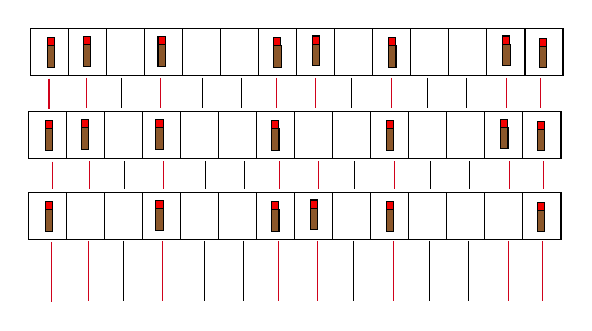
\begin{tikzpicture}[x=0.75pt,y=0.75pt,yscale=-1,xscale=1]
%uncomment if require: \path (0,300); %set diagram left start at 0, and has height of 300

%Shape: Rectangle [id:dp7306471770838919] 
\draw   (193.5,103.24) -- (211.83,103.24) -- (211.83,125.83) -- (193.5,125.83) -- cycle ;
%Shape: Rectangle [id:dp5607628345341253] 
\draw   (211.83,103.24) -- (230.17,103.24) -- (230.17,125.83) -- (211.83,125.83) -- cycle ;
%Shape: Rectangle [id:dp0792661956068278] 
\draw   (230.17,103.24) -- (248.5,103.24) -- (248.5,125.83) -- (230.17,125.83) -- cycle ;
%Shape: Rectangle [id:dp8623895262875295] 
\draw   (248.5,103.24) -- (266.83,103.24) -- (266.83,125.83) -- (248.5,125.83) -- cycle ;
%Shape: Rectangle [id:dp009175660727291923] 
\draw   (266.83,103.24) -- (285.17,103.24) -- (285.17,125.83) -- (266.83,125.83) -- cycle ;
%Shape: Rectangle [id:dp4729260459269564] 
\draw   (285.17,103.24) -- (303.5,103.24) -- (303.5,125.83) -- (285.17,125.83) -- cycle ;
%Shape: Rectangle [id:dp4530702176374507] 
\draw   (303.5,103.24) -- (321.83,103.24) -- (321.83,125.83) -- (303.5,125.83) -- cycle ;
%Shape: Rectangle [id:dp18274736433593486] 
\draw   (321.83,103.24) -- (340.17,103.24) -- (340.17,125.83) -- (321.83,125.83) -- cycle ;
%Shape: Rectangle [id:dp6454813939338947] 
\draw   (340.17,103.24) -- (358.5,103.24) -- (358.5,125.83) -- (340.17,125.83) -- cycle ;
%Shape: Rectangle [id:dp44415589930378796] 
\draw   (358.5,103.24) -- (376.83,103.24) -- (376.83,125.83) -- (358.5,125.83) -- cycle ;
%Shape: Rectangle [id:dp44316809627896814] 
\draw   (376.83,103.24) -- (395.17,103.24) -- (395.17,125.83) -- (376.83,125.83) -- cycle ;
%Shape: Rectangle [id:dp3768823609089883] 
\draw   (395.17,103.24) -- (413.5,103.24) -- (413.5,125.83) -- (395.17,125.83) -- cycle ;
%Shape: Rectangle [id:dp2370210201858336] 
\draw   (413.5,103.24) -- (431.83,103.24) -- (431.83,125.83) -- (413.5,125.83) -- cycle ;
%Shape: Rectangle [id:dp4899807962812457] 
\draw   (431.83,103.24) -- (450.17,103.24) -- (450.17,125.83) -- (431.83,125.83) -- cycle ;
%Shape: Rectangle [id:dp4368680678750193] 
\draw  [fill={rgb, 255:red, 139; green, 87; blue, 42 }  ,fill opacity=1 ] (201.67,111.58) -- (205.33,111.58) -- (205.33,122) -- (201.67,122) -- cycle ;
%Shape: Rectangle [id:dp09500539877263525] 
\draw  [fill={rgb, 255:red, 244; green, 0; blue, 0 }  ,fill opacity=1 ] (201.67,107.67) -- (205.17,107.67) -- (205.17,111.58) -- (201.67,111.58) -- cycle ;
%Shape: Rectangle [id:dp1483728050123183] 
\draw  [fill={rgb, 255:red, 139; green, 87; blue, 42 }  ,fill opacity=1 ] (219,111.25) -- (222.67,111.25) -- (222.67,121.67) -- (219,121.67) -- cycle ;
%Shape: Rectangle [id:dp593349582542728] 
\draw  [fill={rgb, 255:red, 244; green, 0; blue, 0 }  ,fill opacity=1 ] (219,107.33) -- (222.5,107.33) -- (222.5,111.25) -- (219,111.25) -- cycle ;
%Shape: Rectangle [id:dp4070158701487039] 
\draw  [fill={rgb, 255:red, 139; green, 87; blue, 42 }  ,fill opacity=1 ] (255,111.25) -- (258.67,111.25) -- (258.67,121.67) -- (255,121.67) -- cycle ;
%Shape: Rectangle [id:dp4458058453343535] 
\draw  [fill={rgb, 255:red, 244; green, 0; blue, 0 }  ,fill opacity=1 ] (255,107.33) -- (258.5,107.33) -- (258.5,111.25) -- (255,111.25) -- cycle ;
%Shape: Rectangle [id:dp9277371430125845] 
\draw  [fill={rgb, 255:red, 139; green, 87; blue, 42 }  ,fill opacity=1 ] (438.67,111.92) -- (442.33,111.92) -- (442.33,122.33) -- (438.67,122.33) -- cycle ;
%Shape: Rectangle [id:dp3082228602345055] 
\draw  [fill={rgb, 255:red, 244; green, 0; blue, 0 }  ,fill opacity=1 ] (438.67,108) -- (442.17,108) -- (442.17,111.92) -- (438.67,111.92) -- cycle ;
%Shape: Rectangle [id:dp17154116631501037] 
\draw  [fill={rgb, 255:red, 139; green, 87; blue, 42 }  ,fill opacity=1 ] (310.67,111.58) -- (314.33,111.58) -- (314.33,122) -- (310.67,122) -- cycle ;
%Shape: Rectangle [id:dp6278512827702475] 
\draw  [fill={rgb, 255:red, 244; green, 0; blue, 0 }  ,fill opacity=1 ] (310.67,107.67) -- (314.17,107.67) -- (314.17,111.58) -- (310.67,111.58) -- cycle ;
%Shape: Rectangle [id:dp31389089597210484] 
\draw  [fill={rgb, 255:red, 139; green, 87; blue, 42 }  ,fill opacity=1 ] (329.33,110.92) -- (333,110.92) -- (333,121.33) -- (329.33,121.33) -- cycle ;
%Shape: Rectangle [id:dp3848680259197699] 
\draw  [fill={rgb, 255:red, 244; green, 0; blue, 0 }  ,fill opacity=1 ] (329.33,107) -- (332.83,107) -- (332.83,110.92) -- (329.33,110.92) -- cycle ;
%Shape: Rectangle [id:dp6018543086688013] 
\draw  [fill={rgb, 255:red, 139; green, 87; blue, 42 }  ,fill opacity=1 ] (366,111.58) -- (369.67,111.58) -- (369.67,122) -- (366,122) -- cycle ;
%Shape: Rectangle [id:dp599252549604423] 
\draw  [fill={rgb, 255:red, 244; green, 0; blue, 0 }  ,fill opacity=1 ] (366,107.67) -- (369.5,107.67) -- (369.5,111.58) -- (366,111.58) -- cycle ;
%Shape: Rectangle [id:dp9476241971366911] 
\draw  [fill={rgb, 255:red, 139; green, 87; blue, 42 }  ,fill opacity=1 ] (421,110.92) -- (424.67,110.92) -- (424.67,121.33) -- (421,121.33) -- cycle ;
%Shape: Rectangle [id:dp6884535278941168] 
\draw  [fill={rgb, 255:red, 244; green, 0; blue, 0 }  ,fill opacity=1 ] (421,107) -- (424.5,107) -- (424.5,110.92) -- (421,110.92) -- cycle ;
%Shape: Rectangle [id:dp21310684225387844] 
\draw   (192.5,143.24) -- (210.83,143.24) -- (210.83,165.83) -- (192.5,165.83) -- cycle ;
%Shape: Rectangle [id:dp15308541080894023] 
\draw   (210.83,143.24) -- (229.17,143.24) -- (229.17,165.83) -- (210.83,165.83) -- cycle ;
%Shape: Rectangle [id:dp7369128603266555] 
\draw   (229.17,143.24) -- (247.5,143.24) -- (247.5,165.83) -- (229.17,165.83) -- cycle ;
%Shape: Rectangle [id:dp08559110440629836] 
\draw   (247.5,143.24) -- (265.83,143.24) -- (265.83,165.83) -- (247.5,165.83) -- cycle ;
%Shape: Rectangle [id:dp14775457548619686] 
\draw   (265.83,143.24) -- (284.17,143.24) -- (284.17,165.83) -- (265.83,165.83) -- cycle ;
%Shape: Rectangle [id:dp3380965502807922] 
\draw   (284.17,143.24) -- (302.5,143.24) -- (302.5,165.83) -- (284.17,165.83) -- cycle ;
%Shape: Rectangle [id:dp04351713499783527] 
\draw   (302.5,143.24) -- (320.83,143.24) -- (320.83,165.83) -- (302.5,165.83) -- cycle ;
%Shape: Rectangle [id:dp13842235101866918] 
\draw   (320.83,143.24) -- (339.17,143.24) -- (339.17,165.83) -- (320.83,165.83) -- cycle ;
%Shape: Rectangle [id:dp899528791244269] 
\draw   (339.17,143.24) -- (357.5,143.24) -- (357.5,165.83) -- (339.17,165.83) -- cycle ;
%Shape: Rectangle [id:dp6918354352356124] 
\draw   (357.5,143.24) -- (375.83,143.24) -- (375.83,165.83) -- (357.5,165.83) -- cycle ;
%Shape: Rectangle [id:dp25235294258499197] 
\draw   (375.83,143.24) -- (394.17,143.24) -- (394.17,165.83) -- (375.83,165.83) -- cycle ;
%Shape: Rectangle [id:dp28869943259524966] 
\draw   (394.17,143.24) -- (412.5,143.24) -- (412.5,165.83) -- (394.17,165.83) -- cycle ;
%Shape: Rectangle [id:dp07934088847037046] 
\draw   (412.5,143.24) -- (430.83,143.24) -- (430.83,165.83) -- (412.5,165.83) -- cycle ;
%Shape: Rectangle [id:dp46470597708034844] 
\draw   (430.83,143.24) -- (449.17,143.24) -- (449.17,165.83) -- (430.83,165.83) -- cycle ;
%Shape: Rectangle [id:dp04901031477430984] 
\draw  [fill={rgb, 255:red, 139; green, 87; blue, 42 }  ,fill opacity=1 ] (200.67,151.58) -- (204.33,151.58) -- (204.33,162) -- (200.67,162) -- cycle ;
%Shape: Rectangle [id:dp24013735270779224] 
\draw  [fill={rgb, 255:red, 244; green, 0; blue, 0 }  ,fill opacity=1 ] (200.67,147.67) -- (204.17,147.67) -- (204.17,151.58) -- (200.67,151.58) -- cycle ;
%Shape: Rectangle [id:dp3732303325269448] 
\draw  [fill={rgb, 255:red, 139; green, 87; blue, 42 }  ,fill opacity=1 ] (218,151.25) -- (221.67,151.25) -- (221.67,161.67) -- (218,161.67) -- cycle ;
%Shape: Rectangle [id:dp2562802987887275] 
\draw  [fill={rgb, 255:red, 244; green, 0; blue, 0 }  ,fill opacity=1 ] (218,147.33) -- (221.5,147.33) -- (221.5,151.25) -- (218,151.25) -- cycle ;
%Shape: Rectangle [id:dp9262202162888669] 
\draw  [fill={rgb, 255:red, 139; green, 87; blue, 42 }  ,fill opacity=1 ] (254,151.25) -- (257.67,151.25) -- (257.67,161.67) -- (254,161.67) -- cycle ;
%Shape: Rectangle [id:dp7111698984131953] 
\draw  [fill={rgb, 255:red, 244; green, 0; blue, 0 }  ,fill opacity=1 ] (254,147.33) -- (257.5,147.33) -- (257.5,151.25) -- (254,151.25) -- cycle ;
%Shape: Rectangle [id:dp6100628938411732] 
\draw  [fill={rgb, 255:red, 139; green, 87; blue, 42 }  ,fill opacity=1 ] (437.67,151.92) -- (441.33,151.92) -- (441.33,162.33) -- (437.67,162.33) -- cycle ;
%Shape: Rectangle [id:dp3984678192626203] 
\draw  [fill={rgb, 255:red, 244; green, 0; blue, 0 }  ,fill opacity=1 ] (437.67,148) -- (441.17,148) -- (441.17,151.92) -- (437.67,151.92) -- cycle ;
%Shape: Rectangle [id:dp5088329182863778] 
\draw  [fill={rgb, 255:red, 139; green, 87; blue, 42 }  ,fill opacity=1 ] (309.67,151.58) -- (313.33,151.58) -- (313.33,162) -- (309.67,162) -- cycle ;
%Shape: Rectangle [id:dp7660558191775368] 
\draw  [fill={rgb, 255:red, 244; green, 0; blue, 0 }  ,fill opacity=1 ] (309.67,147.67) -- (313.17,147.67) -- (313.17,151.58) -- (309.67,151.58) -- cycle ;
%Shape: Rectangle [id:dp6967450219158551] 
\draw  [fill={rgb, 255:red, 139; green, 87; blue, 42 }  ,fill opacity=1 ] (365,151.58) -- (368.67,151.58) -- (368.67,162) -- (365,162) -- cycle ;
%Shape: Rectangle [id:dp2672105385631931] 
\draw  [fill={rgb, 255:red, 244; green, 0; blue, 0 }  ,fill opacity=1 ] (365,147.67) -- (368.5,147.67) -- (368.5,151.58) -- (365,151.58) -- cycle ;
%Shape: Rectangle [id:dp1772934340190394] 
\draw  [fill={rgb, 255:red, 139; green, 87; blue, 42 }  ,fill opacity=1 ] (420,150.92) -- (423.67,150.92) -- (423.67,161.33) -- (420,161.33) -- cycle ;
%Shape: Rectangle [id:dp33718367695896434] 
\draw  [fill={rgb, 255:red, 244; green, 0; blue, 0 }  ,fill opacity=1 ] (420,147) -- (423.5,147) -- (423.5,150.92) -- (420,150.92) -- cycle ;
%Shape: Rectangle [id:dp29973241992445065] 
\draw   (192.5,182.24) -- (210.83,182.24) -- (210.83,204.83) -- (192.5,204.83) -- cycle ;
%Shape: Rectangle [id:dp915797441388662] 
\draw   (210.83,182.24) -- (229.17,182.24) -- (229.17,204.83) -- (210.83,204.83) -- cycle ;
%Shape: Rectangle [id:dp6972498895193435] 
\draw   (229.17,182.24) -- (247.5,182.24) -- (247.5,204.83) -- (229.17,204.83) -- cycle ;
%Shape: Rectangle [id:dp5185032478559118] 
\draw   (247.5,182.24) -- (265.83,182.24) -- (265.83,204.83) -- (247.5,204.83) -- cycle ;
%Shape: Rectangle [id:dp8211606146424363] 
\draw   (265.83,182.24) -- (284.17,182.24) -- (284.17,204.83) -- (265.83,204.83) -- cycle ;
%Shape: Rectangle [id:dp8023896256315195] 
\draw   (284.17,182.24) -- (302.5,182.24) -- (302.5,204.83) -- (284.17,204.83) -- cycle ;
%Shape: Rectangle [id:dp49891219038392] 
\draw   (302.5,182.24) -- (320.83,182.24) -- (320.83,204.83) -- (302.5,204.83) -- cycle ;
%Shape: Rectangle [id:dp6600654029349139] 
\draw   (320.83,182.24) -- (339.17,182.24) -- (339.17,204.83) -- (320.83,204.83) -- cycle ;
%Shape: Rectangle [id:dp11318057620216593] 
\draw   (339.17,182.24) -- (357.5,182.24) -- (357.5,204.83) -- (339.17,204.83) -- cycle ;
%Shape: Rectangle [id:dp3744427953209425] 
\draw   (357.5,182.24) -- (375.83,182.24) -- (375.83,204.83) -- (357.5,204.83) -- cycle ;
%Shape: Rectangle [id:dp7781448276038074] 
\draw   (375.83,182.24) -- (394.17,182.24) -- (394.17,204.83) -- (375.83,204.83) -- cycle ;
%Shape: Rectangle [id:dp26100874258401796] 
\draw   (394.17,182.24) -- (412.5,182.24) -- (412.5,204.83) -- (394.17,204.83) -- cycle ;
%Shape: Rectangle [id:dp5443536940350958] 
\draw   (412.5,182.24) -- (430.83,182.24) -- (430.83,204.83) -- (412.5,204.83) -- cycle ;
%Shape: Rectangle [id:dp18514199414344035] 
\draw   (430.83,182.24) -- (449.17,182.24) -- (449.17,204.83) -- (430.83,204.83) -- cycle ;
%Shape: Rectangle [id:dp3844083761325583] 
\draw  [fill={rgb, 255:red, 139; green, 87; blue, 42 }  ,fill opacity=1 ] (200.67,190.58) -- (204.33,190.58) -- (204.33,201) -- (200.67,201) -- cycle ;
%Shape: Rectangle [id:dp5665839783950843] 
\draw  [fill={rgb, 255:red, 244; green, 0; blue, 0 }  ,fill opacity=1 ] (200.67,186.67) -- (204.17,186.67) -- (204.17,190.58) -- (200.67,190.58) -- cycle ;
%Shape: Rectangle [id:dp9876904276652537] 
\draw  [fill={rgb, 255:red, 139; green, 87; blue, 42 }  ,fill opacity=1 ] (254,190.25) -- (257.67,190.25) -- (257.67,200.67) -- (254,200.67) -- cycle ;
%Shape: Rectangle [id:dp7048696327315455] 
\draw  [fill={rgb, 255:red, 244; green, 0; blue, 0 }  ,fill opacity=1 ] (254,186.33) -- (257.5,186.33) -- (257.5,190.25) -- (254,190.25) -- cycle ;
%Shape: Rectangle [id:dp932349242304357] 
\draw  [fill={rgb, 255:red, 139; green, 87; blue, 42 }  ,fill opacity=1 ] (437.67,190.92) -- (441.33,190.92) -- (441.33,201.33) -- (437.67,201.33) -- cycle ;
%Shape: Rectangle [id:dp26533668662176735] 
\draw  [fill={rgb, 255:red, 244; green, 0; blue, 0 }  ,fill opacity=1 ] (437.67,187) -- (441.17,187) -- (441.17,190.92) -- (437.67,190.92) -- cycle ;
%Shape: Rectangle [id:dp02695980007818577] 
\draw  [fill={rgb, 255:red, 139; green, 87; blue, 42 }  ,fill opacity=1 ] (309.67,190.58) -- (313.33,190.58) -- (313.33,201) -- (309.67,201) -- cycle ;
%Shape: Rectangle [id:dp3114497357209295] 
\draw  [fill={rgb, 255:red, 244; green, 0; blue, 0 }  ,fill opacity=1 ] (309.67,186.67) -- (313.17,186.67) -- (313.17,190.58) -- (309.67,190.58) -- cycle ;
%Shape: Rectangle [id:dp44348697279949933] 
\draw  [fill={rgb, 255:red, 139; green, 87; blue, 42 }  ,fill opacity=1 ] (328.33,189.92) -- (332,189.92) -- (332,200.33) -- (328.33,200.33) -- cycle ;
%Shape: Rectangle [id:dp3784124318707486] 
\draw  [fill={rgb, 255:red, 244; green, 0; blue, 0 }  ,fill opacity=1 ] (328.33,186) -- (331.83,186) -- (331.83,189.92) -- (328.33,189.92) -- cycle ;
%Shape: Rectangle [id:dp5578954048184986] 
\draw  [fill={rgb, 255:red, 139; green, 87; blue, 42 }  ,fill opacity=1 ] (365,190.58) -- (368.67,190.58) -- (368.67,201) -- (365,201) -- cycle ;
%Shape: Rectangle [id:dp736526795021232] 
\draw  [fill={rgb, 255:red, 244; green, 0; blue, 0 }  ,fill opacity=1 ] (365,186.67) -- (368.5,186.67) -- (368.5,190.58) -- (365,190.58) -- cycle ;
%Straight Lines [id:da23211869104100902] 
\draw [color={rgb, 255:red, 208; green, 2; blue, 27 }  ,draw opacity=1 ]   (202.5,127.51) -- (202.5,142.25) ;
%Straight Lines [id:da8546808588977279] 
\draw [color={rgb, 255:red, 208; green, 2; blue, 27 }  ,draw opacity=1 ]   (220.5,127.17) -- (220.5,141.91) ;
%Straight Lines [id:da3824640222126928] 
\draw [color={rgb, 255:red, 208; green, 2; blue, 27 }  ,draw opacity=1 ]   (256.17,127.17) -- (256.17,141.91) ;
%Straight Lines [id:da09491083254970156] 
\draw [color={rgb, 255:red, 208; green, 2; blue, 27 }  ,draw opacity=1 ]   (312.17,127.17) -- (312.17,141.91) ;
%Straight Lines [id:da9363882317980852] 
\draw [color={rgb, 255:red, 208; green, 2; blue, 27 }  ,draw opacity=1 ]   (330.83,127.17) -- (330.83,141.91) ;
%Straight Lines [id:da9347730048440243] 
\draw [color={rgb, 255:red, 208; green, 2; blue, 27 }  ,draw opacity=1 ]   (367.5,127.17) -- (367.5,141.91) ;
%Straight Lines [id:da07199374823755988] 
\draw [color={rgb, 255:red, 208; green, 2; blue, 27 }  ,draw opacity=1 ]   (422.83,127.17) -- (422.83,141.91) ;
%Straight Lines [id:da8369064287295007] 
\draw [color={rgb, 255:red, 208; green, 2; blue, 27 }  ,draw opacity=1 ]   (439.17,127.17) -- (439.17,141.91) ;
%Straight Lines [id:da9687846894711664] 
\draw [color={rgb, 255:red, 0; green, 0; blue, 0 }  ,draw opacity=1 ]   (237.5,127.17) -- (237.5,141.91) ;
%Straight Lines [id:da1053078374886558] 
\draw [color={rgb, 255:red, 0; green, 0; blue, 0 }  ,draw opacity=1 ]   (276.5,127.17) -- (276.5,141.91) ;
%Straight Lines [id:da14518946834087554] 
\draw [color={rgb, 255:red, 0; green, 0; blue, 0 }  ,draw opacity=1 ]   (295.17,127.17) -- (295.17,141.91) ;
%Straight Lines [id:da13997986323087297] 
\draw [color={rgb, 255:red, 0; green, 0; blue, 0 }  ,draw opacity=1 ]   (348.17,127.17) -- (348.17,141.91) ;
%Straight Lines [id:da48066390457899655] 
\draw [color={rgb, 255:red, 0; green, 0; blue, 0 }  ,draw opacity=1 ]   (384.83,127.17) -- (384.83,141.91) ;
%Straight Lines [id:da1833109680307854] 
\draw [color={rgb, 255:red, 0; green, 0; blue, 0 }  ,draw opacity=1 ]   (403.5,127.17) -- (403.5,141.91) ;
%Straight Lines [id:da0842061548753219] 
\draw [color={rgb, 255:red, 208; green, 2; blue, 27 }  ,draw opacity=1 ]   (204,167.56) -- (204,180.83) ;
%Straight Lines [id:da5693275302640379] 
\draw [color={rgb, 255:red, 208; green, 2; blue, 27 }  ,draw opacity=1 ]   (222,167.25) -- (222,180.53) ;
%Straight Lines [id:da9260157648671437] 
\draw [color={rgb, 255:red, 208; green, 2; blue, 27 }  ,draw opacity=1 ]   (257.67,167.25) -- (257.67,180.53) ;
%Straight Lines [id:da7868167529159288] 
\draw [color={rgb, 255:red, 208; green, 2; blue, 27 }  ,draw opacity=1 ]   (313.67,167.25) -- (313.67,180.53) ;
%Straight Lines [id:da11529691283139021] 
\draw [color={rgb, 255:red, 208; green, 2; blue, 27 }  ,draw opacity=1 ]   (332.33,167.25) -- (332.33,180.53) ;
%Straight Lines [id:da003598362247238862] 
\draw [color={rgb, 255:red, 208; green, 2; blue, 27 }  ,draw opacity=1 ]   (369,167.25) -- (369,180.53) ;
%Straight Lines [id:da30207664809868606] 
\draw [color={rgb, 255:red, 208; green, 2; blue, 27 }  ,draw opacity=1 ]   (424.33,167.25) -- (424.33,180.53) ;
%Straight Lines [id:da04843766616282663] 
\draw [color={rgb, 255:red, 208; green, 2; blue, 27 }  ,draw opacity=1 ]   (440.67,167.25) -- (440.67,180.53) ;
%Straight Lines [id:da4114023079704151] 
\draw [color={rgb, 255:red, 0; green, 0; blue, 0 }  ,draw opacity=1 ]   (239,167.25) -- (239,180.53) ;
%Straight Lines [id:da45796431254340697] 
\draw [color={rgb, 255:red, 0; green, 0; blue, 0 }  ,draw opacity=1 ]   (278,167.25) -- (278,180.53) ;
%Straight Lines [id:da2398752999686985] 
\draw [color={rgb, 255:red, 0; green, 0; blue, 0 }  ,draw opacity=1 ]   (296.67,167.25) -- (296.67,180.53) ;
%Straight Lines [id:da7637595687990975] 
\draw [color={rgb, 255:red, 0; green, 0; blue, 0 }  ,draw opacity=1 ]   (349.67,167.25) -- (349.67,180.53) ;
%Straight Lines [id:da15944293707367208] 
\draw [color={rgb, 255:red, 0; green, 0; blue, 0 }  ,draw opacity=1 ]   (386.33,167.25) -- (386.33,180.53) ;
%Straight Lines [id:da024716190660356796] 
\draw [color={rgb, 255:red, 0; green, 0; blue, 0 }  ,draw opacity=1 ]   (405,167.25) -- (405,180.53) ;
%Straight Lines [id:da15205363545917838] 
\draw [color={rgb, 255:red, 208; green, 2; blue, 27 }  ,draw opacity=1 ]   (203.5,206.33) -- (203.5,235.33) ;
%Straight Lines [id:da8962203946781292] 
\draw [color={rgb, 255:red, 208; green, 2; blue, 27 }  ,draw opacity=1 ]   (221.5,205.67) -- (221.5,234.67) ;
%Straight Lines [id:da09314359066526023] 
\draw [color={rgb, 255:red, 208; green, 2; blue, 27 }  ,draw opacity=1 ]   (257.17,205.67) -- (257.17,234.67) ;
%Straight Lines [id:da8654695122762754] 
\draw [color={rgb, 255:red, 208; green, 2; blue, 27 }  ,draw opacity=1 ]   (313.17,205.67) -- (313.17,234.67) ;
%Straight Lines [id:da4669058494925922] 
\draw [color={rgb, 255:red, 208; green, 2; blue, 27 }  ,draw opacity=1 ]   (331.83,205.67) -- (331.83,234.67) ;
%Straight Lines [id:da0798743126470347] 
\draw [color={rgb, 255:red, 208; green, 2; blue, 27 }  ,draw opacity=1 ]   (368.5,205.67) -- (368.5,234.67) ;
%Straight Lines [id:da5633813976729091] 
\draw [color={rgb, 255:red, 208; green, 2; blue, 27 }  ,draw opacity=1 ]   (423.83,205.67) -- (423.83,234.67) ;
%Straight Lines [id:da3088242002339415] 
\draw [color={rgb, 255:red, 208; green, 2; blue, 27 }  ,draw opacity=1 ]   (440.17,205.67) -- (440.17,234.67) ;
%Straight Lines [id:da6769940585144782] 
\draw [color={rgb, 255:red, 0; green, 0; blue, 0 }  ,draw opacity=1 ]   (238.5,205.67) -- (238.5,234.67) ;
%Straight Lines [id:da026908125696294194] 
\draw [color={rgb, 255:red, 0; green, 0; blue, 0 }  ,draw opacity=1 ]   (277.5,205.67) -- (277.5,234.67) ;
%Straight Lines [id:da6155289648900006] 
\draw [color={rgb, 255:red, 0; green, 0; blue, 0 }  ,draw opacity=1 ]   (296.17,205.67) -- (296.17,234.67) ;
%Straight Lines [id:da31010444849639074] 
\draw [color={rgb, 255:red, 0; green, 0; blue, 0 }  ,draw opacity=1 ]   (349.17,205.67) -- (349.17,234.67) ;
%Straight Lines [id:da4943047111870168] 
\draw [color={rgb, 255:red, 0; green, 0; blue, 0 }  ,draw opacity=1 ]   (385.83,205.67) -- (385.83,234.67) ;
%Straight Lines [id:da5225948396237124] 
\draw [color={rgb, 255:red, 0; green, 0; blue, 0 }  ,draw opacity=1 ]   (404.5,205.67) -- (404.5,234.67) ;




\end{tikzpicture}

				}         
				\begin{itemize}
					\item We can see right away that simply running wires underneath every line, using a \textbf{bus}, won't work at all. We'll just get all the 'on' bits at once!
				\end{itemize}				    	
             	
             \end{frame}
             
             \begin{frame}
             	\frametitle{ROM in Minecraft}
             	\begin{itemize}
             		\item We need a way to get the data from one of these lines at a time. Is this reminding you of a circuit you've built before?
             	\end{itemize}
             	
             	{
             	\centering
             	

\tikzset{every picture/.style={line width=0.75pt}} %set default line width to 0.75pt        

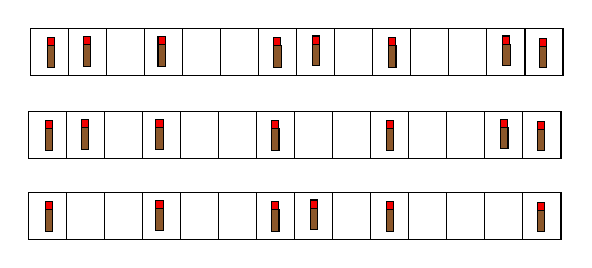
\begin{tikzpicture}[x=0.75pt,y=0.75pt,yscale=-1,xscale=1]
%uncomment if require: \path (0,300); %set diagram left start at 0, and has height of 300

%Shape: Rectangle [id:dp7306471770838919] 
\draw   (193.5,103.24) -- (211.83,103.24) -- (211.83,125.83) -- (193.5,125.83) -- cycle ;
%Shape: Rectangle [id:dp5607628345341253] 
\draw   (211.83,103.24) -- (230.17,103.24) -- (230.17,125.83) -- (211.83,125.83) -- cycle ;
%Shape: Rectangle [id:dp0792661956068278] 
\draw   (230.17,103.24) -- (248.5,103.24) -- (248.5,125.83) -- (230.17,125.83) -- cycle ;
%Shape: Rectangle [id:dp8623895262875295] 
\draw   (248.5,103.24) -- (266.83,103.24) -- (266.83,125.83) -- (248.5,125.83) -- cycle ;
%Shape: Rectangle [id:dp009175660727291923] 
\draw   (266.83,103.24) -- (285.17,103.24) -- (285.17,125.83) -- (266.83,125.83) -- cycle ;
%Shape: Rectangle [id:dp4729260459269564] 
\draw   (285.17,103.24) -- (303.5,103.24) -- (303.5,125.83) -- (285.17,125.83) -- cycle ;
%Shape: Rectangle [id:dp4530702176374507] 
\draw   (303.5,103.24) -- (321.83,103.24) -- (321.83,125.83) -- (303.5,125.83) -- cycle ;
%Shape: Rectangle [id:dp18274736433593486] 
\draw   (321.83,103.24) -- (340.17,103.24) -- (340.17,125.83) -- (321.83,125.83) -- cycle ;
%Shape: Rectangle [id:dp6454813939338947] 
\draw   (340.17,103.24) -- (358.5,103.24) -- (358.5,125.83) -- (340.17,125.83) -- cycle ;
%Shape: Rectangle [id:dp44415589930378796] 
\draw   (358.5,103.24) -- (376.83,103.24) -- (376.83,125.83) -- (358.5,125.83) -- cycle ;
%Shape: Rectangle [id:dp44316809627896814] 
\draw   (376.83,103.24) -- (395.17,103.24) -- (395.17,125.83) -- (376.83,125.83) -- cycle ;
%Shape: Rectangle [id:dp3768823609089883] 
\draw   (395.17,103.24) -- (413.5,103.24) -- (413.5,125.83) -- (395.17,125.83) -- cycle ;
%Shape: Rectangle [id:dp2370210201858336] 
\draw   (413.5,103.24) -- (431.83,103.24) -- (431.83,125.83) -- (413.5,125.83) -- cycle ;
%Shape: Rectangle [id:dp4899807962812457] 
\draw   (431.83,103.24) -- (450.17,103.24) -- (450.17,125.83) -- (431.83,125.83) -- cycle ;
%Shape: Rectangle [id:dp4368680678750193] 
\draw  [fill={rgb, 255:red, 139; green, 87; blue, 42 }  ,fill opacity=1 ] (201.67,111.58) -- (205.33,111.58) -- (205.33,122) -- (201.67,122) -- cycle ;
%Shape: Rectangle [id:dp09500539877263525] 
\draw  [fill={rgb, 255:red, 244; green, 0; blue, 0 }  ,fill opacity=1 ] (201.67,107.67) -- (205.17,107.67) -- (205.17,111.58) -- (201.67,111.58) -- cycle ;
%Shape: Rectangle [id:dp1483728050123183] 
\draw  [fill={rgb, 255:red, 139; green, 87; blue, 42 }  ,fill opacity=1 ] (219,111.25) -- (222.67,111.25) -- (222.67,121.67) -- (219,121.67) -- cycle ;
%Shape: Rectangle [id:dp593349582542728] 
\draw  [fill={rgb, 255:red, 244; green, 0; blue, 0 }  ,fill opacity=1 ] (219,107.33) -- (222.5,107.33) -- (222.5,111.25) -- (219,111.25) -- cycle ;
%Shape: Rectangle [id:dp4070158701487039] 
\draw  [fill={rgb, 255:red, 139; green, 87; blue, 42 }  ,fill opacity=1 ] (255,111.25) -- (258.67,111.25) -- (258.67,121.67) -- (255,121.67) -- cycle ;
%Shape: Rectangle [id:dp4458058453343535] 
\draw  [fill={rgb, 255:red, 244; green, 0; blue, 0 }  ,fill opacity=1 ] (255,107.33) -- (258.5,107.33) -- (258.5,111.25) -- (255,111.25) -- cycle ;
%Shape: Rectangle [id:dp9277371430125845] 
\draw  [fill={rgb, 255:red, 139; green, 87; blue, 42 }  ,fill opacity=1 ] (438.67,111.92) -- (442.33,111.92) -- (442.33,122.33) -- (438.67,122.33) -- cycle ;
%Shape: Rectangle [id:dp3082228602345055] 
\draw  [fill={rgb, 255:red, 244; green, 0; blue, 0 }  ,fill opacity=1 ] (438.67,108) -- (442.17,108) -- (442.17,111.92) -- (438.67,111.92) -- cycle ;
%Shape: Rectangle [id:dp17154116631501037] 
\draw  [fill={rgb, 255:red, 139; green, 87; blue, 42 }  ,fill opacity=1 ] (310.67,111.58) -- (314.33,111.58) -- (314.33,122) -- (310.67,122) -- cycle ;
%Shape: Rectangle [id:dp6278512827702475] 
\draw  [fill={rgb, 255:red, 244; green, 0; blue, 0 }  ,fill opacity=1 ] (310.67,107.67) -- (314.17,107.67) -- (314.17,111.58) -- (310.67,111.58) -- cycle ;
%Shape: Rectangle [id:dp31389089597210484] 
\draw  [fill={rgb, 255:red, 139; green, 87; blue, 42 }  ,fill opacity=1 ] (329.33,110.92) -- (333,110.92) -- (333,121.33) -- (329.33,121.33) -- cycle ;
%Shape: Rectangle [id:dp3848680259197699] 
\draw  [fill={rgb, 255:red, 244; green, 0; blue, 0 }  ,fill opacity=1 ] (329.33,107) -- (332.83,107) -- (332.83,110.92) -- (329.33,110.92) -- cycle ;
%Shape: Rectangle [id:dp6018543086688013] 
\draw  [fill={rgb, 255:red, 139; green, 87; blue, 42 }  ,fill opacity=1 ] (366,111.58) -- (369.67,111.58) -- (369.67,122) -- (366,122) -- cycle ;
%Shape: Rectangle [id:dp599252549604423] 
\draw  [fill={rgb, 255:red, 244; green, 0; blue, 0 }  ,fill opacity=1 ] (366,107.67) -- (369.5,107.67) -- (369.5,111.58) -- (366,111.58) -- cycle ;
%Shape: Rectangle [id:dp9476241971366911] 
\draw  [fill={rgb, 255:red, 139; green, 87; blue, 42 }  ,fill opacity=1 ] (421,110.92) -- (424.67,110.92) -- (424.67,121.33) -- (421,121.33) -- cycle ;
%Shape: Rectangle [id:dp6884535278941168] 
\draw  [fill={rgb, 255:red, 244; green, 0; blue, 0 }  ,fill opacity=1 ] (421,107) -- (424.5,107) -- (424.5,110.92) -- (421,110.92) -- cycle ;
%Shape: Rectangle [id:dp21310684225387844] 
\draw   (192.5,143.24) -- (210.83,143.24) -- (210.83,165.83) -- (192.5,165.83) -- cycle ;
%Shape: Rectangle [id:dp15308541080894023] 
\draw   (210.83,143.24) -- (229.17,143.24) -- (229.17,165.83) -- (210.83,165.83) -- cycle ;
%Shape: Rectangle [id:dp7369128603266555] 
\draw   (229.17,143.24) -- (247.5,143.24) -- (247.5,165.83) -- (229.17,165.83) -- cycle ;
%Shape: Rectangle [id:dp08559110440629836] 
\draw   (247.5,143.24) -- (265.83,143.24) -- (265.83,165.83) -- (247.5,165.83) -- cycle ;
%Shape: Rectangle [id:dp14775457548619686] 
\draw   (265.83,143.24) -- (284.17,143.24) -- (284.17,165.83) -- (265.83,165.83) -- cycle ;
%Shape: Rectangle [id:dp3380965502807922] 
\draw   (284.17,143.24) -- (302.5,143.24) -- (302.5,165.83) -- (284.17,165.83) -- cycle ;
%Shape: Rectangle [id:dp04351713499783527] 
\draw   (302.5,143.24) -- (320.83,143.24) -- (320.83,165.83) -- (302.5,165.83) -- cycle ;
%Shape: Rectangle [id:dp13842235101866918] 
\draw   (320.83,143.24) -- (339.17,143.24) -- (339.17,165.83) -- (320.83,165.83) -- cycle ;
%Shape: Rectangle [id:dp899528791244269] 
\draw   (339.17,143.24) -- (357.5,143.24) -- (357.5,165.83) -- (339.17,165.83) -- cycle ;
%Shape: Rectangle [id:dp6918354352356124] 
\draw   (357.5,143.24) -- (375.83,143.24) -- (375.83,165.83) -- (357.5,165.83) -- cycle ;
%Shape: Rectangle [id:dp25235294258499197] 
\draw   (375.83,143.24) -- (394.17,143.24) -- (394.17,165.83) -- (375.83,165.83) -- cycle ;
%Shape: Rectangle [id:dp28869943259524966] 
\draw   (394.17,143.24) -- (412.5,143.24) -- (412.5,165.83) -- (394.17,165.83) -- cycle ;
%Shape: Rectangle [id:dp07934088847037046] 
\draw   (412.5,143.24) -- (430.83,143.24) -- (430.83,165.83) -- (412.5,165.83) -- cycle ;
%Shape: Rectangle [id:dp46470597708034844] 
\draw   (430.83,143.24) -- (449.17,143.24) -- (449.17,165.83) -- (430.83,165.83) -- cycle ;
%Shape: Rectangle [id:dp04901031477430984] 
\draw  [fill={rgb, 255:red, 139; green, 87; blue, 42 }  ,fill opacity=1 ] (200.67,151.58) -- (204.33,151.58) -- (204.33,162) -- (200.67,162) -- cycle ;
%Shape: Rectangle [id:dp24013735270779224] 
\draw  [fill={rgb, 255:red, 244; green, 0; blue, 0 }  ,fill opacity=1 ] (200.67,147.67) -- (204.17,147.67) -- (204.17,151.58) -- (200.67,151.58) -- cycle ;
%Shape: Rectangle [id:dp3732303325269448] 
\draw  [fill={rgb, 255:red, 139; green, 87; blue, 42 }  ,fill opacity=1 ] (218,151.25) -- (221.67,151.25) -- (221.67,161.67) -- (218,161.67) -- cycle ;
%Shape: Rectangle [id:dp2562802987887275] 
\draw  [fill={rgb, 255:red, 244; green, 0; blue, 0 }  ,fill opacity=1 ] (218,147.33) -- (221.5,147.33) -- (221.5,151.25) -- (218,151.25) -- cycle ;
%Shape: Rectangle [id:dp9262202162888669] 
\draw  [fill={rgb, 255:red, 139; green, 87; blue, 42 }  ,fill opacity=1 ] (254,151.25) -- (257.67,151.25) -- (257.67,161.67) -- (254,161.67) -- cycle ;
%Shape: Rectangle [id:dp7111698984131953] 
\draw  [fill={rgb, 255:red, 244; green, 0; blue, 0 }  ,fill opacity=1 ] (254,147.33) -- (257.5,147.33) -- (257.5,151.25) -- (254,151.25) -- cycle ;
%Shape: Rectangle [id:dp6100628938411732] 
\draw  [fill={rgb, 255:red, 139; green, 87; blue, 42 }  ,fill opacity=1 ] (437.67,151.92) -- (441.33,151.92) -- (441.33,162.33) -- (437.67,162.33) -- cycle ;
%Shape: Rectangle [id:dp3984678192626203] 
\draw  [fill={rgb, 255:red, 244; green, 0; blue, 0 }  ,fill opacity=1 ] (437.67,148) -- (441.17,148) -- (441.17,151.92) -- (437.67,151.92) -- cycle ;
%Shape: Rectangle [id:dp5088329182863778] 
\draw  [fill={rgb, 255:red, 139; green, 87; blue, 42 }  ,fill opacity=1 ] (309.67,151.58) -- (313.33,151.58) -- (313.33,162) -- (309.67,162) -- cycle ;
%Shape: Rectangle [id:dp7660558191775368] 
\draw  [fill={rgb, 255:red, 244; green, 0; blue, 0 }  ,fill opacity=1 ] (309.67,147.67) -- (313.17,147.67) -- (313.17,151.58) -- (309.67,151.58) -- cycle ;
%Shape: Rectangle [id:dp6967450219158551] 
\draw  [fill={rgb, 255:red, 139; green, 87; blue, 42 }  ,fill opacity=1 ] (365,151.58) -- (368.67,151.58) -- (368.67,162) -- (365,162) -- cycle ;
%Shape: Rectangle [id:dp2672105385631931] 
\draw  [fill={rgb, 255:red, 244; green, 0; blue, 0 }  ,fill opacity=1 ] (365,147.67) -- (368.5,147.67) -- (368.5,151.58) -- (365,151.58) -- cycle ;
%Shape: Rectangle [id:dp1772934340190394] 
\draw  [fill={rgb, 255:red, 139; green, 87; blue, 42 }  ,fill opacity=1 ] (420,150.92) -- (423.67,150.92) -- (423.67,161.33) -- (420,161.33) -- cycle ;
%Shape: Rectangle [id:dp33718367695896434] 
\draw  [fill={rgb, 255:red, 244; green, 0; blue, 0 }  ,fill opacity=1 ] (420,147) -- (423.5,147) -- (423.5,150.92) -- (420,150.92) -- cycle ;
%Shape: Rectangle [id:dp29973241992445065] 
\draw   (192.5,182.24) -- (210.83,182.24) -- (210.83,204.83) -- (192.5,204.83) -- cycle ;
%Shape: Rectangle [id:dp915797441388662] 
\draw   (210.83,182.24) -- (229.17,182.24) -- (229.17,204.83) -- (210.83,204.83) -- cycle ;
%Shape: Rectangle [id:dp6972498895193435] 
\draw   (229.17,182.24) -- (247.5,182.24) -- (247.5,204.83) -- (229.17,204.83) -- cycle ;
%Shape: Rectangle [id:dp5185032478559118] 
\draw   (247.5,182.24) -- (265.83,182.24) -- (265.83,204.83) -- (247.5,204.83) -- cycle ;
%Shape: Rectangle [id:dp8211606146424363] 
\draw   (265.83,182.24) -- (284.17,182.24) -- (284.17,204.83) -- (265.83,204.83) -- cycle ;
%Shape: Rectangle [id:dp8023896256315195] 
\draw   (284.17,182.24) -- (302.5,182.24) -- (302.5,204.83) -- (284.17,204.83) -- cycle ;
%Shape: Rectangle [id:dp49891219038392] 
\draw   (302.5,182.24) -- (320.83,182.24) -- (320.83,204.83) -- (302.5,204.83) -- cycle ;
%Shape: Rectangle [id:dp6600654029349139] 
\draw   (320.83,182.24) -- (339.17,182.24) -- (339.17,204.83) -- (320.83,204.83) -- cycle ;
%Shape: Rectangle [id:dp11318057620216593] 
\draw   (339.17,182.24) -- (357.5,182.24) -- (357.5,204.83) -- (339.17,204.83) -- cycle ;
%Shape: Rectangle [id:dp3744427953209425] 
\draw   (357.5,182.24) -- (375.83,182.24) -- (375.83,204.83) -- (357.5,204.83) -- cycle ;
%Shape: Rectangle [id:dp7781448276038074] 
\draw   (375.83,182.24) -- (394.17,182.24) -- (394.17,204.83) -- (375.83,204.83) -- cycle ;
%Shape: Rectangle [id:dp26100874258401796] 
\draw   (394.17,182.24) -- (412.5,182.24) -- (412.5,204.83) -- (394.17,204.83) -- cycle ;
%Shape: Rectangle [id:dp5443536940350958] 
\draw   (412.5,182.24) -- (430.83,182.24) -- (430.83,204.83) -- (412.5,204.83) -- cycle ;
%Shape: Rectangle [id:dp18514199414344035] 
\draw   (430.83,182.24) -- (449.17,182.24) -- (449.17,204.83) -- (430.83,204.83) -- cycle ;
%Shape: Rectangle [id:dp3844083761325583] 
\draw  [fill={rgb, 255:red, 139; green, 87; blue, 42 }  ,fill opacity=1 ] (200.67,190.58) -- (204.33,190.58) -- (204.33,201) -- (200.67,201) -- cycle ;
%Shape: Rectangle [id:dp5665839783950843] 
\draw  [fill={rgb, 255:red, 244; green, 0; blue, 0 }  ,fill opacity=1 ] (200.67,186.67) -- (204.17,186.67) -- (204.17,190.58) -- (200.67,190.58) -- cycle ;
%Shape: Rectangle [id:dp9876904276652537] 
\draw  [fill={rgb, 255:red, 139; green, 87; blue, 42 }  ,fill opacity=1 ] (254,190.25) -- (257.67,190.25) -- (257.67,200.67) -- (254,200.67) -- cycle ;
%Shape: Rectangle [id:dp7048696327315455] 
\draw  [fill={rgb, 255:red, 244; green, 0; blue, 0 }  ,fill opacity=1 ] (254,186.33) -- (257.5,186.33) -- (257.5,190.25) -- (254,190.25) -- cycle ;
%Shape: Rectangle [id:dp932349242304357] 
\draw  [fill={rgb, 255:red, 139; green, 87; blue, 42 }  ,fill opacity=1 ] (437.67,190.92) -- (441.33,190.92) -- (441.33,201.33) -- (437.67,201.33) -- cycle ;
%Shape: Rectangle [id:dp26533668662176735] 
\draw  [fill={rgb, 255:red, 244; green, 0; blue, 0 }  ,fill opacity=1 ] (437.67,187) -- (441.17,187) -- (441.17,190.92) -- (437.67,190.92) -- cycle ;
%Shape: Rectangle [id:dp02695980007818577] 
\draw  [fill={rgb, 255:red, 139; green, 87; blue, 42 }  ,fill opacity=1 ] (309.67,190.58) -- (313.33,190.58) -- (313.33,201) -- (309.67,201) -- cycle ;
%Shape: Rectangle [id:dp3114497357209295] 
\draw  [fill={rgb, 255:red, 244; green, 0; blue, 0 }  ,fill opacity=1 ] (309.67,186.67) -- (313.17,186.67) -- (313.17,190.58) -- (309.67,190.58) -- cycle ;
%Shape: Rectangle [id:dp44348697279949933] 
\draw  [fill={rgb, 255:red, 139; green, 87; blue, 42 }  ,fill opacity=1 ] (328.33,189.92) -- (332,189.92) -- (332,200.33) -- (328.33,200.33) -- cycle ;
%Shape: Rectangle [id:dp3784124318707486] 
\draw  [fill={rgb, 255:red, 244; green, 0; blue, 0 }  ,fill opacity=1 ] (328.33,186) -- (331.83,186) -- (331.83,189.92) -- (328.33,189.92) -- cycle ;
%Shape: Rectangle [id:dp5578954048184986] 
\draw  [fill={rgb, 255:red, 139; green, 87; blue, 42 }  ,fill opacity=1 ] (365,190.58) -- (368.67,190.58) -- (368.67,201) -- (365,201) -- cycle ;
%Shape: Rectangle [id:dp736526795021232] 
\draw  [fill={rgb, 255:red, 244; green, 0; blue, 0 }  ,fill opacity=1 ] (365,186.67) -- (368.5,186.67) -- (368.5,190.58) -- (365,190.58) -- cycle ;




\end{tikzpicture}


             	}
             	
             	
             	\begin{itemize}
             		\item Think about where else you've seen long parallel rows of blocks with torches!
             	\end{itemize}
             	
             \end{frame}
             
             \begin{frame}
             	\frametitle{ROM in Minecraft}
             	\begin{itemize}
             		\item That's right- you can use a decoder!
             		\item Specifically, we want a binary to decimal decoder.
             		\item We'll explain why in a minute.
             		
             	\end{itemize}
             \end{frame}
             
             \begin{frame}
             	\frametitle{ROM in Minecraft}
             	{
             	\centering
             	

\tikzset{every picture/.style={line width=0.75pt}} %set default line width to 0.75pt        

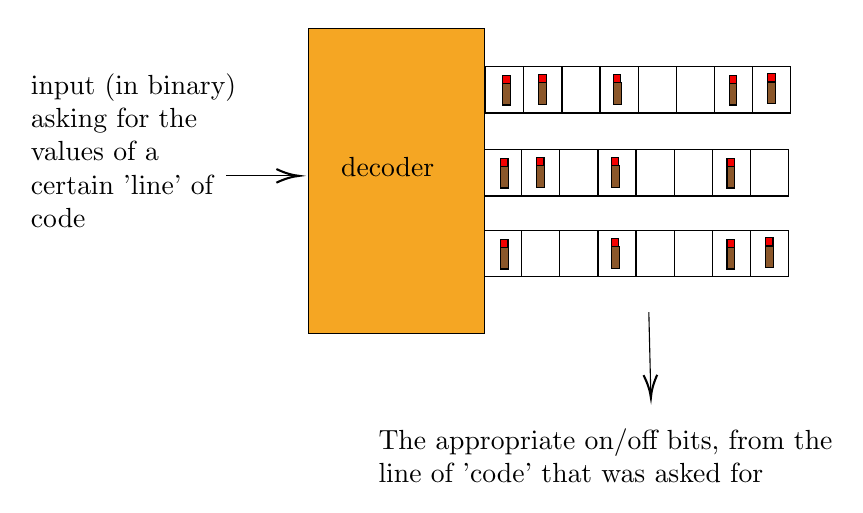
\begin{tikzpicture}[x=0.75pt,y=0.75pt,yscale=-1,xscale=1]
%uncomment if require: \path (0,300); %set diagram left start at 0, and has height of 300

%Shape: Rectangle [id:dp7306471770838919] 
\draw   (276,54.24) -- (294.33,54.24) -- (294.33,76.83) -- (276,76.83) -- cycle ;
%Shape: Rectangle [id:dp5607628345341253] 
\draw   (294.33,54.24) -- (312.67,54.24) -- (312.67,76.83) -- (294.33,76.83) -- cycle ;
%Shape: Rectangle [id:dp0792661956068278] 
\draw   (312.67,54.24) -- (331,54.24) -- (331,76.83) -- (312.67,76.83) -- cycle ;
%Shape: Rectangle [id:dp8623895262875295] 
\draw   (331,54.24) -- (349.33,54.24) -- (349.33,76.83) -- (331,76.83) -- cycle ;
%Shape: Rectangle [id:dp009175660727291923] 
\draw   (349.33,54.24) -- (367.67,54.24) -- (367.67,76.83) -- (349.33,76.83) -- cycle ;
%Shape: Rectangle [id:dp4729260459269564] 
\draw   (367.67,54.24) -- (386,54.24) -- (386,76.83) -- (367.67,76.83) -- cycle ;
%Shape: Rectangle [id:dp4530702176374507] 
\draw   (386,54.24) -- (404.33,54.24) -- (404.33,76.83) -- (386,76.83) -- cycle ;
%Shape: Rectangle [id:dp18274736433593486] 
\draw   (404.33,54.24) -- (422.67,54.24) -- (422.67,76.83) -- (404.33,76.83) -- cycle ;
%Shape: Rectangle [id:dp4368680678750193] 
\draw  [fill={rgb, 255:red, 139; green, 87; blue, 42 }  ,fill opacity=1 ] (284.17,62.58) -- (287.83,62.58) -- (287.83,73) -- (284.17,73) -- cycle ;
%Shape: Rectangle [id:dp09500539877263525] 
\draw  [fill={rgb, 255:red, 244; green, 0; blue, 0 }  ,fill opacity=1 ] (284.17,58.67) -- (287.67,58.67) -- (287.67,62.58) -- (284.17,62.58) -- cycle ;
%Shape: Rectangle [id:dp1483728050123183] 
\draw  [fill={rgb, 255:red, 139; green, 87; blue, 42 }  ,fill opacity=1 ] (301.5,62.25) -- (305.17,62.25) -- (305.17,72.67) -- (301.5,72.67) -- cycle ;
%Shape: Rectangle [id:dp593349582542728] 
\draw  [fill={rgb, 255:red, 244; green, 0; blue, 0 }  ,fill opacity=1 ] (301.5,58.33) -- (305,58.33) -- (305,62.25) -- (301.5,62.25) -- cycle ;
%Shape: Rectangle [id:dp4070158701487039] 
\draw  [fill={rgb, 255:red, 139; green, 87; blue, 42 }  ,fill opacity=1 ] (337.5,62.25) -- (341.17,62.25) -- (341.17,72.67) -- (337.5,72.67) -- cycle ;
%Shape: Rectangle [id:dp4458058453343535] 
\draw  [fill={rgb, 255:red, 244; green, 0; blue, 0 }  ,fill opacity=1 ] (337.5,58.33) -- (341,58.33) -- (341,62.25) -- (337.5,62.25) -- cycle ;
%Shape: Rectangle [id:dp17154116631501037] 
\draw  [fill={rgb, 255:red, 139; green, 87; blue, 42 }  ,fill opacity=1 ] (393.17,62.58) -- (396.83,62.58) -- (396.83,73) -- (393.17,73) -- cycle ;
%Shape: Rectangle [id:dp6278512827702475] 
\draw  [fill={rgb, 255:red, 244; green, 0; blue, 0 }  ,fill opacity=1 ] (393.17,58.67) -- (396.67,58.67) -- (396.67,62.58) -- (393.17,62.58) -- cycle ;
%Shape: Rectangle [id:dp31389089597210484] 
\draw  [fill={rgb, 255:red, 139; green, 87; blue, 42 }  ,fill opacity=1 ] (411.83,61.92) -- (415.5,61.92) -- (415.5,72.33) -- (411.83,72.33) -- cycle ;
%Shape: Rectangle [id:dp3848680259197699] 
\draw  [fill={rgb, 255:red, 244; green, 0; blue, 0 }  ,fill opacity=1 ] (411.83,58) -- (415.33,58) -- (415.33,61.92) -- (411.83,61.92) -- cycle ;
%Shape: Rectangle [id:dp21310684225387844] 
\draw   (275,94.24) -- (293.33,94.24) -- (293.33,116.83) -- (275,116.83) -- cycle ;
%Shape: Rectangle [id:dp15308541080894023] 
\draw   (293.33,94.24) -- (311.67,94.24) -- (311.67,116.83) -- (293.33,116.83) -- cycle ;
%Shape: Rectangle [id:dp7369128603266555] 
\draw   (311.67,94.24) -- (330,94.24) -- (330,116.83) -- (311.67,116.83) -- cycle ;
%Shape: Rectangle [id:dp08559110440629836] 
\draw   (330,94.24) -- (348.33,94.24) -- (348.33,116.83) -- (330,116.83) -- cycle ;
%Shape: Rectangle [id:dp14775457548619686] 
\draw   (348.33,94.24) -- (366.67,94.24) -- (366.67,116.83) -- (348.33,116.83) -- cycle ;
%Shape: Rectangle [id:dp3380965502807922] 
\draw   (366.67,94.24) -- (385,94.24) -- (385,116.83) -- (366.67,116.83) -- cycle ;
%Shape: Rectangle [id:dp04351713499783527] 
\draw   (385,94.24) -- (403.33,94.24) -- (403.33,116.83) -- (385,116.83) -- cycle ;
%Shape: Rectangle [id:dp13842235101866918] 
\draw   (403.33,94.24) -- (421.67,94.24) -- (421.67,116.83) -- (403.33,116.83) -- cycle ;
%Shape: Rectangle [id:dp04901031477430984] 
\draw  [fill={rgb, 255:red, 139; green, 87; blue, 42 }  ,fill opacity=1 ] (283.17,102.58) -- (286.83,102.58) -- (286.83,113) -- (283.17,113) -- cycle ;
%Shape: Rectangle [id:dp24013735270779224] 
\draw  [fill={rgb, 255:red, 244; green, 0; blue, 0 }  ,fill opacity=1 ] (283.17,98.67) -- (286.67,98.67) -- (286.67,102.58) -- (283.17,102.58) -- cycle ;
%Shape: Rectangle [id:dp3732303325269448] 
\draw  [fill={rgb, 255:red, 139; green, 87; blue, 42 }  ,fill opacity=1 ] (300.5,102.25) -- (304.17,102.25) -- (304.17,112.67) -- (300.5,112.67) -- cycle ;
%Shape: Rectangle [id:dp2562802987887275] 
\draw  [fill={rgb, 255:red, 244; green, 0; blue, 0 }  ,fill opacity=1 ] (300.5,98.33) -- (304,98.33) -- (304,102.25) -- (300.5,102.25) -- cycle ;
%Shape: Rectangle [id:dp9262202162888669] 
\draw  [fill={rgb, 255:red, 139; green, 87; blue, 42 }  ,fill opacity=1 ] (336.5,102.25) -- (340.17,102.25) -- (340.17,112.67) -- (336.5,112.67) -- cycle ;
%Shape: Rectangle [id:dp7111698984131953] 
\draw  [fill={rgb, 255:red, 244; green, 0; blue, 0 }  ,fill opacity=1 ] (336.5,98.33) -- (340,98.33) -- (340,102.25) -- (336.5,102.25) -- cycle ;
%Shape: Rectangle [id:dp5088329182863778] 
\draw  [fill={rgb, 255:red, 139; green, 87; blue, 42 }  ,fill opacity=1 ] (392.17,102.58) -- (395.83,102.58) -- (395.83,113) -- (392.17,113) -- cycle ;
%Shape: Rectangle [id:dp7660558191775368] 
\draw  [fill={rgb, 255:red, 244; green, 0; blue, 0 }  ,fill opacity=1 ] (392.17,98.67) -- (395.67,98.67) -- (395.67,102.58) -- (392.17,102.58) -- cycle ;
%Shape: Rectangle [id:dp29973241992445065] 
\draw   (275,133.24) -- (293.33,133.24) -- (293.33,155.83) -- (275,155.83) -- cycle ;
%Shape: Rectangle [id:dp915797441388662] 
\draw   (293.33,133.24) -- (311.67,133.24) -- (311.67,155.83) -- (293.33,155.83) -- cycle ;
%Shape: Rectangle [id:dp6972498895193435] 
\draw   (311.67,133.24) -- (330,133.24) -- (330,155.83) -- (311.67,155.83) -- cycle ;
%Shape: Rectangle [id:dp5185032478559118] 
\draw   (330,133.24) -- (348.33,133.24) -- (348.33,155.83) -- (330,155.83) -- cycle ;
%Shape: Rectangle [id:dp8211606146424363] 
\draw   (348.33,133.24) -- (366.67,133.24) -- (366.67,155.83) -- (348.33,155.83) -- cycle ;
%Shape: Rectangle [id:dp8023896256315195] 
\draw   (366.67,133.24) -- (385,133.24) -- (385,155.83) -- (366.67,155.83) -- cycle ;
%Shape: Rectangle [id:dp49891219038392] 
\draw   (385,133.24) -- (403.33,133.24) -- (403.33,155.83) -- (385,155.83) -- cycle ;
%Shape: Rectangle [id:dp6600654029349139] 
\draw   (403.33,133.24) -- (421.67,133.24) -- (421.67,155.83) -- (403.33,155.83) -- cycle ;
%Shape: Rectangle [id:dp3844083761325583] 
\draw  [fill={rgb, 255:red, 139; green, 87; blue, 42 }  ,fill opacity=1 ] (283.17,141.58) -- (286.83,141.58) -- (286.83,152) -- (283.17,152) -- cycle ;
%Shape: Rectangle [id:dp5665839783950843] 
\draw  [fill={rgb, 255:red, 244; green, 0; blue, 0 }  ,fill opacity=1 ] (283.17,137.67) -- (286.67,137.67) -- (286.67,141.58) -- (283.17,141.58) -- cycle ;
%Shape: Rectangle [id:dp9876904276652537] 
\draw  [fill={rgb, 255:red, 139; green, 87; blue, 42 }  ,fill opacity=1 ] (336.5,141.25) -- (340.17,141.25) -- (340.17,151.67) -- (336.5,151.67) -- cycle ;
%Shape: Rectangle [id:dp7048696327315455] 
\draw  [fill={rgb, 255:red, 244; green, 0; blue, 0 }  ,fill opacity=1 ] (336.5,137.33) -- (340,137.33) -- (340,141.25) -- (336.5,141.25) -- cycle ;
%Shape: Rectangle [id:dp02695980007818577] 
\draw  [fill={rgb, 255:red, 139; green, 87; blue, 42 }  ,fill opacity=1 ] (392.17,141.58) -- (395.83,141.58) -- (395.83,152) -- (392.17,152) -- cycle ;
%Shape: Rectangle [id:dp3114497357209295] 
\draw  [fill={rgb, 255:red, 244; green, 0; blue, 0 }  ,fill opacity=1 ] (392.17,137.67) -- (395.67,137.67) -- (395.67,141.58) -- (392.17,141.58) -- cycle ;
%Shape: Rectangle [id:dp44348697279949933] 
\draw  [fill={rgb, 255:red, 139; green, 87; blue, 42 }  ,fill opacity=1 ] (410.83,140.92) -- (414.5,140.92) -- (414.5,151.33) -- (410.83,151.33) -- cycle ;
%Shape: Rectangle [id:dp3784124318707486] 
\draw  [fill={rgb, 255:red, 244; green, 0; blue, 0 }  ,fill opacity=1 ] (410.83,137) -- (414.33,137) -- (414.33,140.92) -- (410.83,140.92) -- cycle ;
%Shape: Rectangle [id:dp4197232968092024] 
\draw  [fill={rgb, 255:red, 245; green, 166; blue, 35 }  ,fill opacity=1 ] (190.5,36) -- (275.5,36) -- (275.5,183.25) -- (190.5,183.25) -- cycle ;
%Straight Lines [id:da05311225057578406] 
\draw    (151,107.13) -- (184,107.13) ;
\draw [shift={(186,107.13)}, rotate = 180] [color={rgb, 255:red, 0; green, 0; blue, 0 }  ][line width=0.75]    (10.93,-3.29) .. controls (6.95,-1.4) and (3.31,-0.3) .. (0,0) .. controls (3.31,0.3) and (6.95,1.4) .. (10.93,3.29)   ;
%Straight Lines [id:da7015013983266646] 
\draw    (354.5,172.75) -- (355.45,212) ;
\draw [shift={(355.5,214)}, rotate = 268.61] [color={rgb, 255:red, 0; green, 0; blue, 0 }  ][line width=0.75]    (10.93,-3.29) .. controls (6.95,-1.4) and (3.31,-0.3) .. (0,0) .. controls (3.31,0.3) and (6.95,1.4) .. (10.93,3.29)   ;

% Text Node
\draw (205,97) node [anchor=north west][inner sep=0.75pt]   [align=left] {decoder};
% Text Node
\draw (55.5,56.63) node [anchor=north west][inner sep=0.75pt]   [align=left] {input (in binary)\\asking for the\\values of a \\certain 'line' of\\code};
% Text Node
\draw (223,227.5) node [anchor=north west][inner sep=0.75pt]   [align=left] {The appropriate on/off bits, from the\\line of 'code' that was asked for};


\end{tikzpicture}

             	}
             	
             \end{frame}
             
             \begin{frame}
             	\frametitle{ROM in Minecraft}
             	\begin{itemize}
             		\item Why a binary to decimal decoder, though?
             		\begin{itemize}
             			\item You don't know this yet, but it's highly convenient for us to request the line number in \textbf{binary}.
             			\item Our circuit basically says: Here's the line number we're currently at (in binary). Can you get me the data stored in that line of code, please?
             		\end{itemize}
             	\end{itemize}
             \end{frame}
             
             
		\subsection{Interpretation of our Programs}
			
			\begin{frame}
				\frametitle{Interpreting The 'Assembly'}
				\begin{itemize}
					\item Now, we can safely say that we know how to do two things.
					\begin{itemize}
						\item First, we can store multiple lines of 'CMSC389E Assembly Code' using redstone torches and blocks
						\item Second, we can use a binary to decimal decoder to, given a line number, produce the 'line' of code that is stored in our ROM.
					\end{itemize}
					\item This is excellent news, because now all we need is to \textbf{interpret} those lines of code, and we're home free.
				\end{itemize}
			\end{frame}
			
			\begin{frame}
				\frametitle{Interpreting The 'Assembly'}
				\begin{itemize}
					\item Here's what we've got so far. We ask for a line of code, and we get \textbf{14 parallel signals}, representing 14 bits of 389E Assembly
				\end{itemize}
				
				{
				\centering
				

\tikzset{every picture/.style={line width=0.75pt}} %set default line width to 0.75pt        

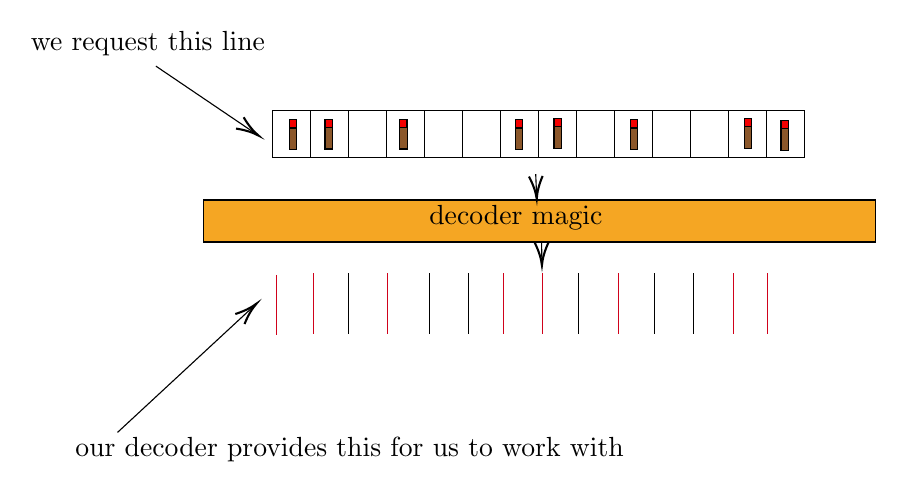
\begin{tikzpicture}[x=0.75pt,y=0.75pt,yscale=-1,xscale=1]
%uncomment if require: \path (0,300); %set diagram left start at 0, and has height of 300

%Shape: Rectangle [id:dp7306471770838919] 
\draw   (203,51.74) -- (221.33,51.74) -- (221.33,74.33) -- (203,74.33) -- cycle ;
%Shape: Rectangle [id:dp5607628345341253] 
\draw   (221.33,51.74) -- (239.67,51.74) -- (239.67,74.33) -- (221.33,74.33) -- cycle ;
%Shape: Rectangle [id:dp0792661956068278] 
\draw   (239.67,51.74) -- (258,51.74) -- (258,74.33) -- (239.67,74.33) -- cycle ;
%Shape: Rectangle [id:dp8623895262875295] 
\draw   (258,51.74) -- (276.33,51.74) -- (276.33,74.33) -- (258,74.33) -- cycle ;
%Shape: Rectangle [id:dp009175660727291923] 
\draw   (276.33,51.74) -- (294.67,51.74) -- (294.67,74.33) -- (276.33,74.33) -- cycle ;
%Shape: Rectangle [id:dp4729260459269564] 
\draw   (294.67,51.74) -- (313,51.74) -- (313,74.33) -- (294.67,74.33) -- cycle ;
%Shape: Rectangle [id:dp4530702176374507] 
\draw   (313,51.74) -- (331.33,51.74) -- (331.33,74.33) -- (313,74.33) -- cycle ;
%Shape: Rectangle [id:dp18274736433593486] 
\draw   (331.33,51.74) -- (349.67,51.74) -- (349.67,74.33) -- (331.33,74.33) -- cycle ;
%Shape: Rectangle [id:dp6454813939338947] 
\draw   (349.67,51.74) -- (368,51.74) -- (368,74.33) -- (349.67,74.33) -- cycle ;
%Shape: Rectangle [id:dp44415589930378796] 
\draw   (368,51.74) -- (386.33,51.74) -- (386.33,74.33) -- (368,74.33) -- cycle ;
%Shape: Rectangle [id:dp44316809627896814] 
\draw   (386.33,51.74) -- (404.67,51.74) -- (404.67,74.33) -- (386.33,74.33) -- cycle ;
%Shape: Rectangle [id:dp3768823609089883] 
\draw   (404.67,51.74) -- (423,51.74) -- (423,74.33) -- (404.67,74.33) -- cycle ;
%Shape: Rectangle [id:dp2370210201858336] 
\draw   (423,51.74) -- (441.33,51.74) -- (441.33,74.33) -- (423,74.33) -- cycle ;
%Shape: Rectangle [id:dp4899807962812457] 
\draw   (441.33,51.74) -- (459.67,51.74) -- (459.67,74.33) -- (441.33,74.33) -- cycle ;
%Shape: Rectangle [id:dp4368680678750193] 
\draw  [fill={rgb, 255:red, 139; green, 87; blue, 42 }  ,fill opacity=1 ] (211.17,60.08) -- (214.83,60.08) -- (214.83,70.5) -- (211.17,70.5) -- cycle ;
%Shape: Rectangle [id:dp09500539877263525] 
\draw  [fill={rgb, 255:red, 244; green, 0; blue, 0 }  ,fill opacity=1 ] (211.17,56.17) -- (214.67,56.17) -- (214.67,60.08) -- (211.17,60.08) -- cycle ;
%Shape: Rectangle [id:dp1483728050123183] 
\draw  [fill={rgb, 255:red, 139; green, 87; blue, 42 }  ,fill opacity=1 ] (228.5,59.75) -- (232.17,59.75) -- (232.17,70.17) -- (228.5,70.17) -- cycle ;
%Shape: Rectangle [id:dp593349582542728] 
\draw  [fill={rgb, 255:red, 244; green, 0; blue, 0 }  ,fill opacity=1 ] (228.5,55.83) -- (232,55.83) -- (232,59.75) -- (228.5,59.75) -- cycle ;
%Shape: Rectangle [id:dp4070158701487039] 
\draw  [fill={rgb, 255:red, 139; green, 87; blue, 42 }  ,fill opacity=1 ] (264.5,59.75) -- (268.17,59.75) -- (268.17,70.17) -- (264.5,70.17) -- cycle ;
%Shape: Rectangle [id:dp4458058453343535] 
\draw  [fill={rgb, 255:red, 244; green, 0; blue, 0 }  ,fill opacity=1 ] (264.5,55.83) -- (268,55.83) -- (268,59.75) -- (264.5,59.75) -- cycle ;
%Shape: Rectangle [id:dp9277371430125845] 
\draw  [fill={rgb, 255:red, 139; green, 87; blue, 42 }  ,fill opacity=1 ] (448.17,60.42) -- (451.83,60.42) -- (451.83,70.83) -- (448.17,70.83) -- cycle ;
%Shape: Rectangle [id:dp3082228602345055] 
\draw  [fill={rgb, 255:red, 244; green, 0; blue, 0 }  ,fill opacity=1 ] (448.17,56.5) -- (451.67,56.5) -- (451.67,60.42) -- (448.17,60.42) -- cycle ;
%Shape: Rectangle [id:dp17154116631501037] 
\draw  [fill={rgb, 255:red, 139; green, 87; blue, 42 }  ,fill opacity=1 ] (320.17,60.08) -- (323.83,60.08) -- (323.83,70.5) -- (320.17,70.5) -- cycle ;
%Shape: Rectangle [id:dp6278512827702475] 
\draw  [fill={rgb, 255:red, 244; green, 0; blue, 0 }  ,fill opacity=1 ] (320.17,56.17) -- (323.67,56.17) -- (323.67,60.08) -- (320.17,60.08) -- cycle ;
%Shape: Rectangle [id:dp31389089597210484] 
\draw  [fill={rgb, 255:red, 139; green, 87; blue, 42 }  ,fill opacity=1 ] (338.83,59.42) -- (342.5,59.42) -- (342.5,69.83) -- (338.83,69.83) -- cycle ;
%Shape: Rectangle [id:dp3848680259197699] 
\draw  [fill={rgb, 255:red, 244; green, 0; blue, 0 }  ,fill opacity=1 ] (338.83,55.5) -- (342.33,55.5) -- (342.33,59.42) -- (338.83,59.42) -- cycle ;
%Shape: Rectangle [id:dp6018543086688013] 
\draw  [fill={rgb, 255:red, 139; green, 87; blue, 42 }  ,fill opacity=1 ] (375.5,60.08) -- (379.17,60.08) -- (379.17,70.5) -- (375.5,70.5) -- cycle ;
%Shape: Rectangle [id:dp599252549604423] 
\draw  [fill={rgb, 255:red, 244; green, 0; blue, 0 }  ,fill opacity=1 ] (375.5,56.17) -- (379,56.17) -- (379,60.08) -- (375.5,60.08) -- cycle ;
%Shape: Rectangle [id:dp9476241971366911] 
\draw  [fill={rgb, 255:red, 139; green, 87; blue, 42 }  ,fill opacity=1 ] (430.5,59.42) -- (434.17,59.42) -- (434.17,69.83) -- (430.5,69.83) -- cycle ;
%Shape: Rectangle [id:dp6884535278941168] 
\draw  [fill={rgb, 255:red, 244; green, 0; blue, 0 }  ,fill opacity=1 ] (430.5,55.5) -- (434,55.5) -- (434,59.42) -- (430.5,59.42) -- cycle ;
%Straight Lines [id:da8130436103927301] 
\draw [color={rgb, 255:red, 208; green, 2; blue, 27 }  ,draw opacity=1 ]   (205,130.83) -- (205,159.83) ;
%Straight Lines [id:da08462131345193069] 
\draw [color={rgb, 255:red, 208; green, 2; blue, 27 }  ,draw opacity=1 ]   (223,130.17) -- (223,159.17) ;
%Straight Lines [id:da8359957829774382] 
\draw [color={rgb, 255:red, 208; green, 2; blue, 27 }  ,draw opacity=1 ]   (258.67,130.17) -- (258.67,159.17) ;
%Straight Lines [id:da3866920597345579] 
\draw [color={rgb, 255:red, 208; green, 2; blue, 27 }  ,draw opacity=1 ]   (314.67,130.17) -- (314.67,159.17) ;
%Straight Lines [id:da5942403939779883] 
\draw [color={rgb, 255:red, 208; green, 2; blue, 27 }  ,draw opacity=1 ]   (333.33,130.17) -- (333.33,159.17) ;
%Straight Lines [id:da22634310425539206] 
\draw [color={rgb, 255:red, 208; green, 2; blue, 27 }  ,draw opacity=1 ]   (370,130.17) -- (370,159.17) ;
%Straight Lines [id:da23791169110885224] 
\draw [color={rgb, 255:red, 208; green, 2; blue, 27 }  ,draw opacity=1 ]   (425.33,130.17) -- (425.33,159.17) ;
%Straight Lines [id:da9365841080673278] 
\draw [color={rgb, 255:red, 208; green, 2; blue, 27 }  ,draw opacity=1 ]   (441.67,130.17) -- (441.67,159.17) ;
%Straight Lines [id:da3945985170381383] 
\draw [color={rgb, 255:red, 0; green, 0; blue, 0 }  ,draw opacity=1 ]   (240,130.17) -- (240,159.17) ;
%Straight Lines [id:da3721123428333971] 
\draw [color={rgb, 255:red, 0; green, 0; blue, 0 }  ,draw opacity=1 ]   (279,130.17) -- (279,159.17) ;
%Straight Lines [id:da013616551740032623] 
\draw [color={rgb, 255:red, 0; green, 0; blue, 0 }  ,draw opacity=1 ]   (297.67,130.17) -- (297.67,159.17) ;
%Straight Lines [id:da9364095553547536] 
\draw [color={rgb, 255:red, 0; green, 0; blue, 0 }  ,draw opacity=1 ]   (350.67,130.17) -- (350.67,159.17) ;
%Straight Lines [id:da7903503951079389] 
\draw [color={rgb, 255:red, 0; green, 0; blue, 0 }  ,draw opacity=1 ]   (387.33,130.17) -- (387.33,159.17) ;
%Straight Lines [id:da6948026493349652] 
\draw [color={rgb, 255:red, 0; green, 0; blue, 0 }  ,draw opacity=1 ]   (406,130.17) -- (406,159.17) ;
%Straight Lines [id:da4088221703357503] 
\draw    (147,30.25) -- (194.84,62.63) ;
\draw [shift={(196.5,63.75)}, rotate = 214.09] [color={rgb, 255:red, 0; green, 0; blue, 0 }  ][line width=0.75]    (10.93,-3.29) .. controls (6.95,-1.4) and (3.31,-0.3) .. (0,0) .. controls (3.31,0.3) and (6.95,1.4) .. (10.93,3.29)   ;
%Straight Lines [id:da9371104688202003] 
\draw    (128.5,206.75) -- (194.03,146.03) ;
\draw [shift={(195.5,144.67)}, rotate = 497.18] [color={rgb, 255:red, 0; green, 0; blue, 0 }  ][line width=0.75]    (10.93,-3.29) .. controls (6.95,-1.4) and (3.31,-0.3) .. (0,0) .. controls (3.31,0.3) and (6.95,1.4) .. (10.93,3.29)   ;
%Shape: Rectangle [id:dp19839900197450522] 
\draw  [fill={rgb, 255:red, 245; green, 166; blue, 35 }  ,fill opacity=1 ] (170,94.75) -- (493.5,94.75) -- (493.5,115) -- (170,115) -- cycle ;
%Straight Lines [id:da7709890896181596] 
\draw    (330,82.25) -- (330.42,92.25) ;
\draw [shift={(330.5,94.25)}, rotate = 267.61] [color={rgb, 255:red, 0; green, 0; blue, 0 }  ][line width=0.75]    (10.93,-3.29) .. controls (6.95,-1.4) and (3.31,-0.3) .. (0,0) .. controls (3.31,0.3) and (6.95,1.4) .. (10.93,3.29)   ;
%Straight Lines [id:da6519792124694934] 
\draw    (332.83,114.67) -- (332.97,124.25) ;
\draw [shift={(333,126.25)}, rotate = 269.18] [color={rgb, 255:red, 0; green, 0; blue, 0 }  ][line width=0.75]    (10.93,-3.29) .. controls (6.95,-1.4) and (3.31,-0.3) .. (0,0) .. controls (3.31,0.3) and (6.95,1.4) .. (10.93,3.29)   ;

% Text Node
\draw (85.5,12) node [anchor=north west][inner sep=0.75pt]   [align=left] {we request this line};
% Text Node
\draw (107,208) node [anchor=north west][inner sep=0.75pt]   [align=left] {our decoder provides this for us to work with};
% Text Node
\draw (277.5,96) node [anchor=north west][inner sep=0.75pt]   [align=left] {decoder magic};


\end{tikzpicture}

				}
				
			\end{frame}
			
			\begin{frame}
				\frametitle{Interpreting The 'Assembly'}
				\begin{itemize}
					\item Okay, so how will we actually 'interpret' these 14 parallel signals of CMSC389E Assembly?
					\item In other words, what will we actually \textit{do} with the signals we have?
					\item That is where our journey ends for now. (The answer lies in the project specification for P5)
					\item I'll talk more about the actual work you have to do to interpret the Assembly lines using an actual circuit once we finish the rest of the pieces of the puzzle (Program Counter + Registers) as well.
				\end{itemize}
			\end{frame}
       
             
            
        
   	
\end{document}
